\documentclass{article}
\usepackage{geometry, graphicx, float, subfigure, amsmath, bm, threeparttable}
\usepackage[marginal]{footmisc}
\geometry{a4paper,scale=0.8}

\title{\bf{pBR322 Mapping by Restriction Digestion with EcoR1/HincII/PvuII and Electrophoresis}}
\author{Xun Zhao (Partner: Samantha)}
\date{March 15, 2019}

\begin{document}
    \begin{titlepage}
        \maketitle
        \setcounter{page}{0}
        \thispagestyle{empty}
    \end{titlepage}

    \renewcommand{\abstractname}{Introduction}
    \begin{abstract}
        In order to defend the attack from virus, some bacterias can produce enzymes to digest invasive DNA molecule of virus. Among these kinds of enzymes, some of them cut DNA randomly, while others called restriction enzymes only cut at specific sequence. Thus, we can use these enzymes to digest the plasmid and get DNA fragments with different length. 

        As the cut sites are fixed in a plasmid, we can reconstruct the relative positions of restriction sites of a plasmid, called mapping.

        Firstly, we digest the plasmid with all possible combinations of 3 restriction enzymes. Then, we can use the agarose gel and certain voltage to separate negatively charged DNA fragments and use loading dye to indicate their positions under UV. And their travel distances are proportional to the reciprocal of logarithm of the number of base pairs, namely, the size of molecule compared with the size of holes in gel, which allows us to draw a standard curve from a reference plasmid with known structure. Finally, we can get the length from travel distance based on the standard curve and use these length to rebuild a plasmid.
    \end{abstract}

    \section{Results}
        \subsection{Raw Result Photo}
            To make the photo more readable, I convert\footnote{All the picture analysis below is based on the \textit{Fiji ImageJ}, including color converting and distance measuring.}
            the photo to black-and-white, adjust the contrast and label 9 wells.
            \begin{figure}[H]
                \centering
                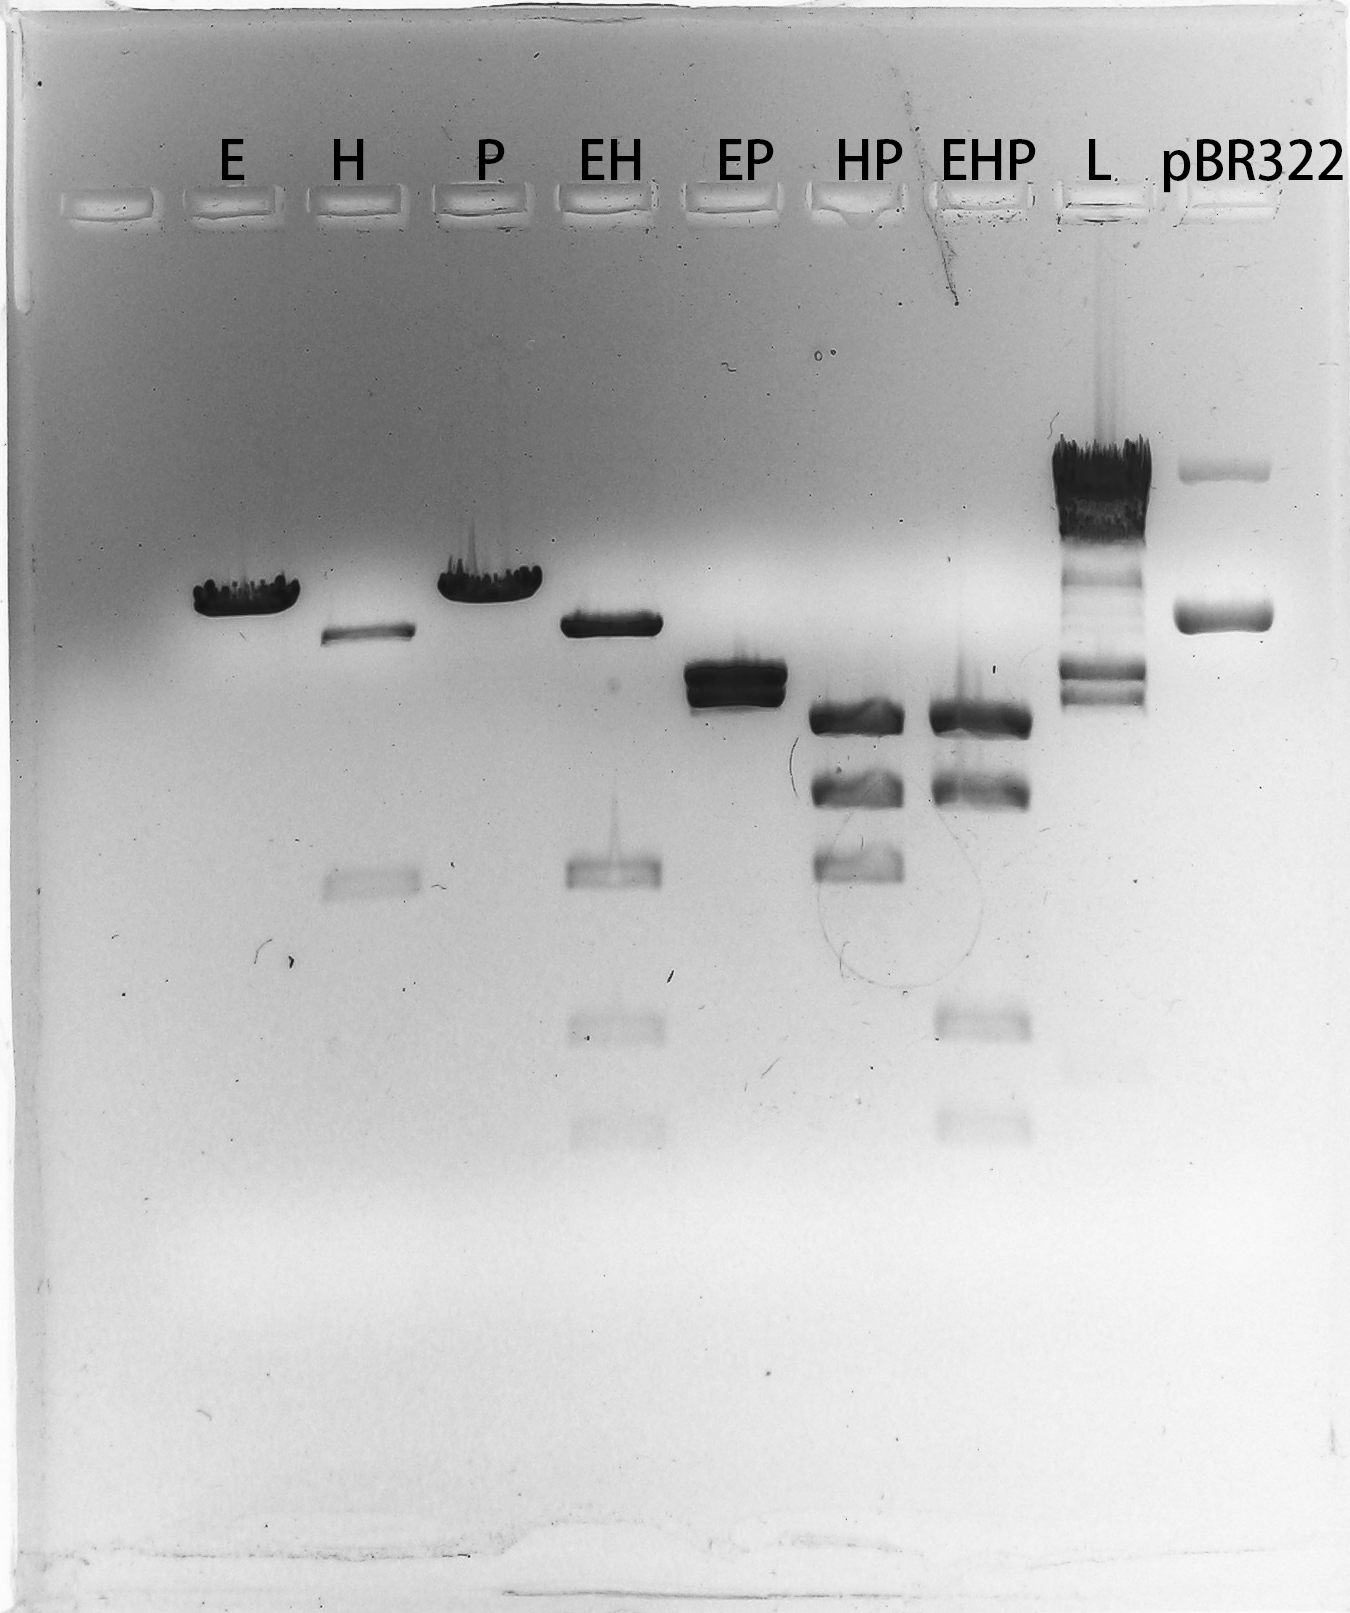
\includegraphics[width = 0.5\textwidth]{../Data/xun_and_sam.png}
                \caption{Raw Gel Photo}
            \end{figure}

        \subsection{\boldmath$\lambda\ $\unboldmath DNA Data}
            Here is the known information of $\lambda$ DNA's fragments bands digested by \textbf{HindIII}, which is the $8^{\text{th}}$ well in the photo named {\bf{L}}.

            \begin{table}[H]
                \caption{$\lambda\ $DNA Data}
                \centering
                \begin{tabular}{|l|c|c|r|}
                    \hline
                    &base pairs&log(bps)&distance (pixels)\\
                    \hline
                    1&      23130&4.364175633&266\\
                    2&      9461&3.97386645&292\\
                    3&      6557&3.816705184&326\\
                    4&      4361&3.639586087&376\\
                    5&      2322&3.365862215&468\\
                    6&      2027&3.306853749&502\\
                    7&      564&2.751279104&870\\
                    \hline
                \end{tabular}
                \label{l.data}
            \end{table}

        \subsection{Standard Curve}

            We can write distance in terms of $d$, and base pairs in terms of $n$. According to the relationship, we will have,

            $$d \propto \frac{1}{log(n)}$$

            The raw curve is plotted as follows,
            \begin{figure}[H]
                \centering
                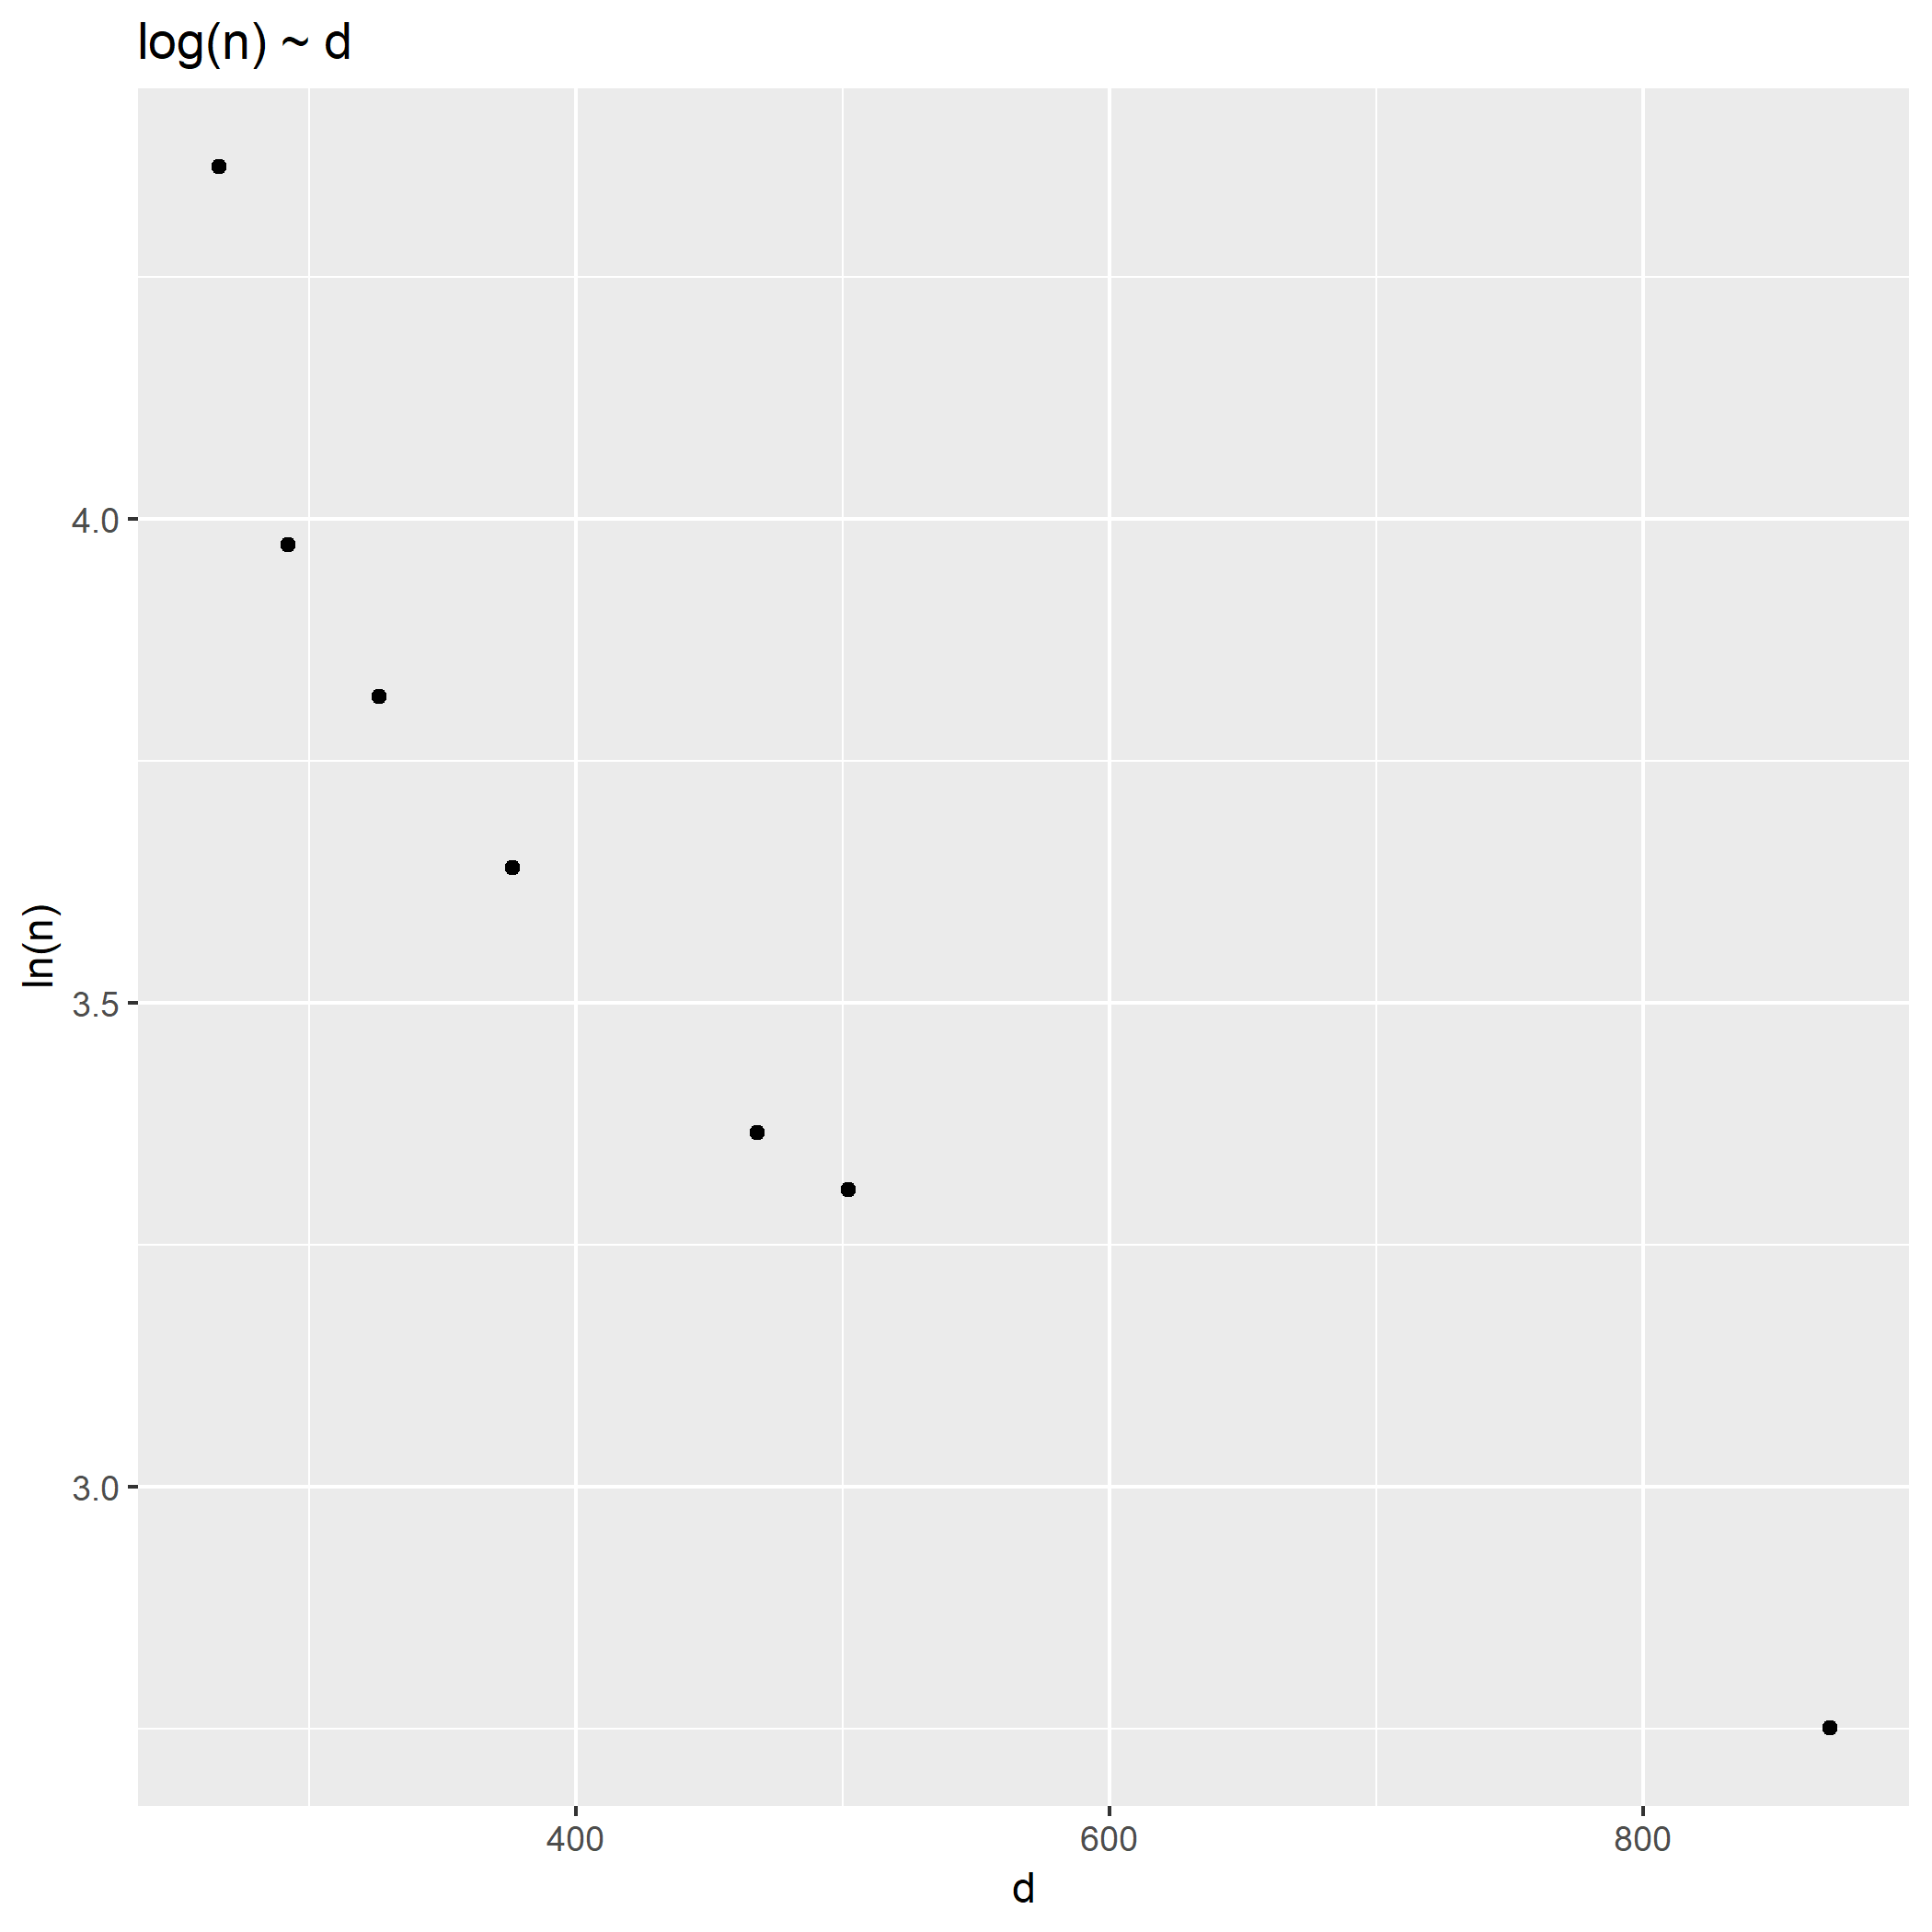
\includegraphics[width = 0.4\textwidth]{../Data/raw_point.png}
                \caption{The realtionship between distance and logarithm of number of base pairs}
                \label{raw.curve}
            \end{figure}

            After choosing some of the data points and using linear regression fitting algorithm, I derived the equation that:
            $$n = exp(4.2 - 1.7 \times 10 ^ {-3} \cdot d)$$
            where $n$ is the length (bps) of DNA fragments and $d$ is the distance these fragments travel.

            The combination of this line and data points is as follows,
            \begin{figure}[H]
                \centering
                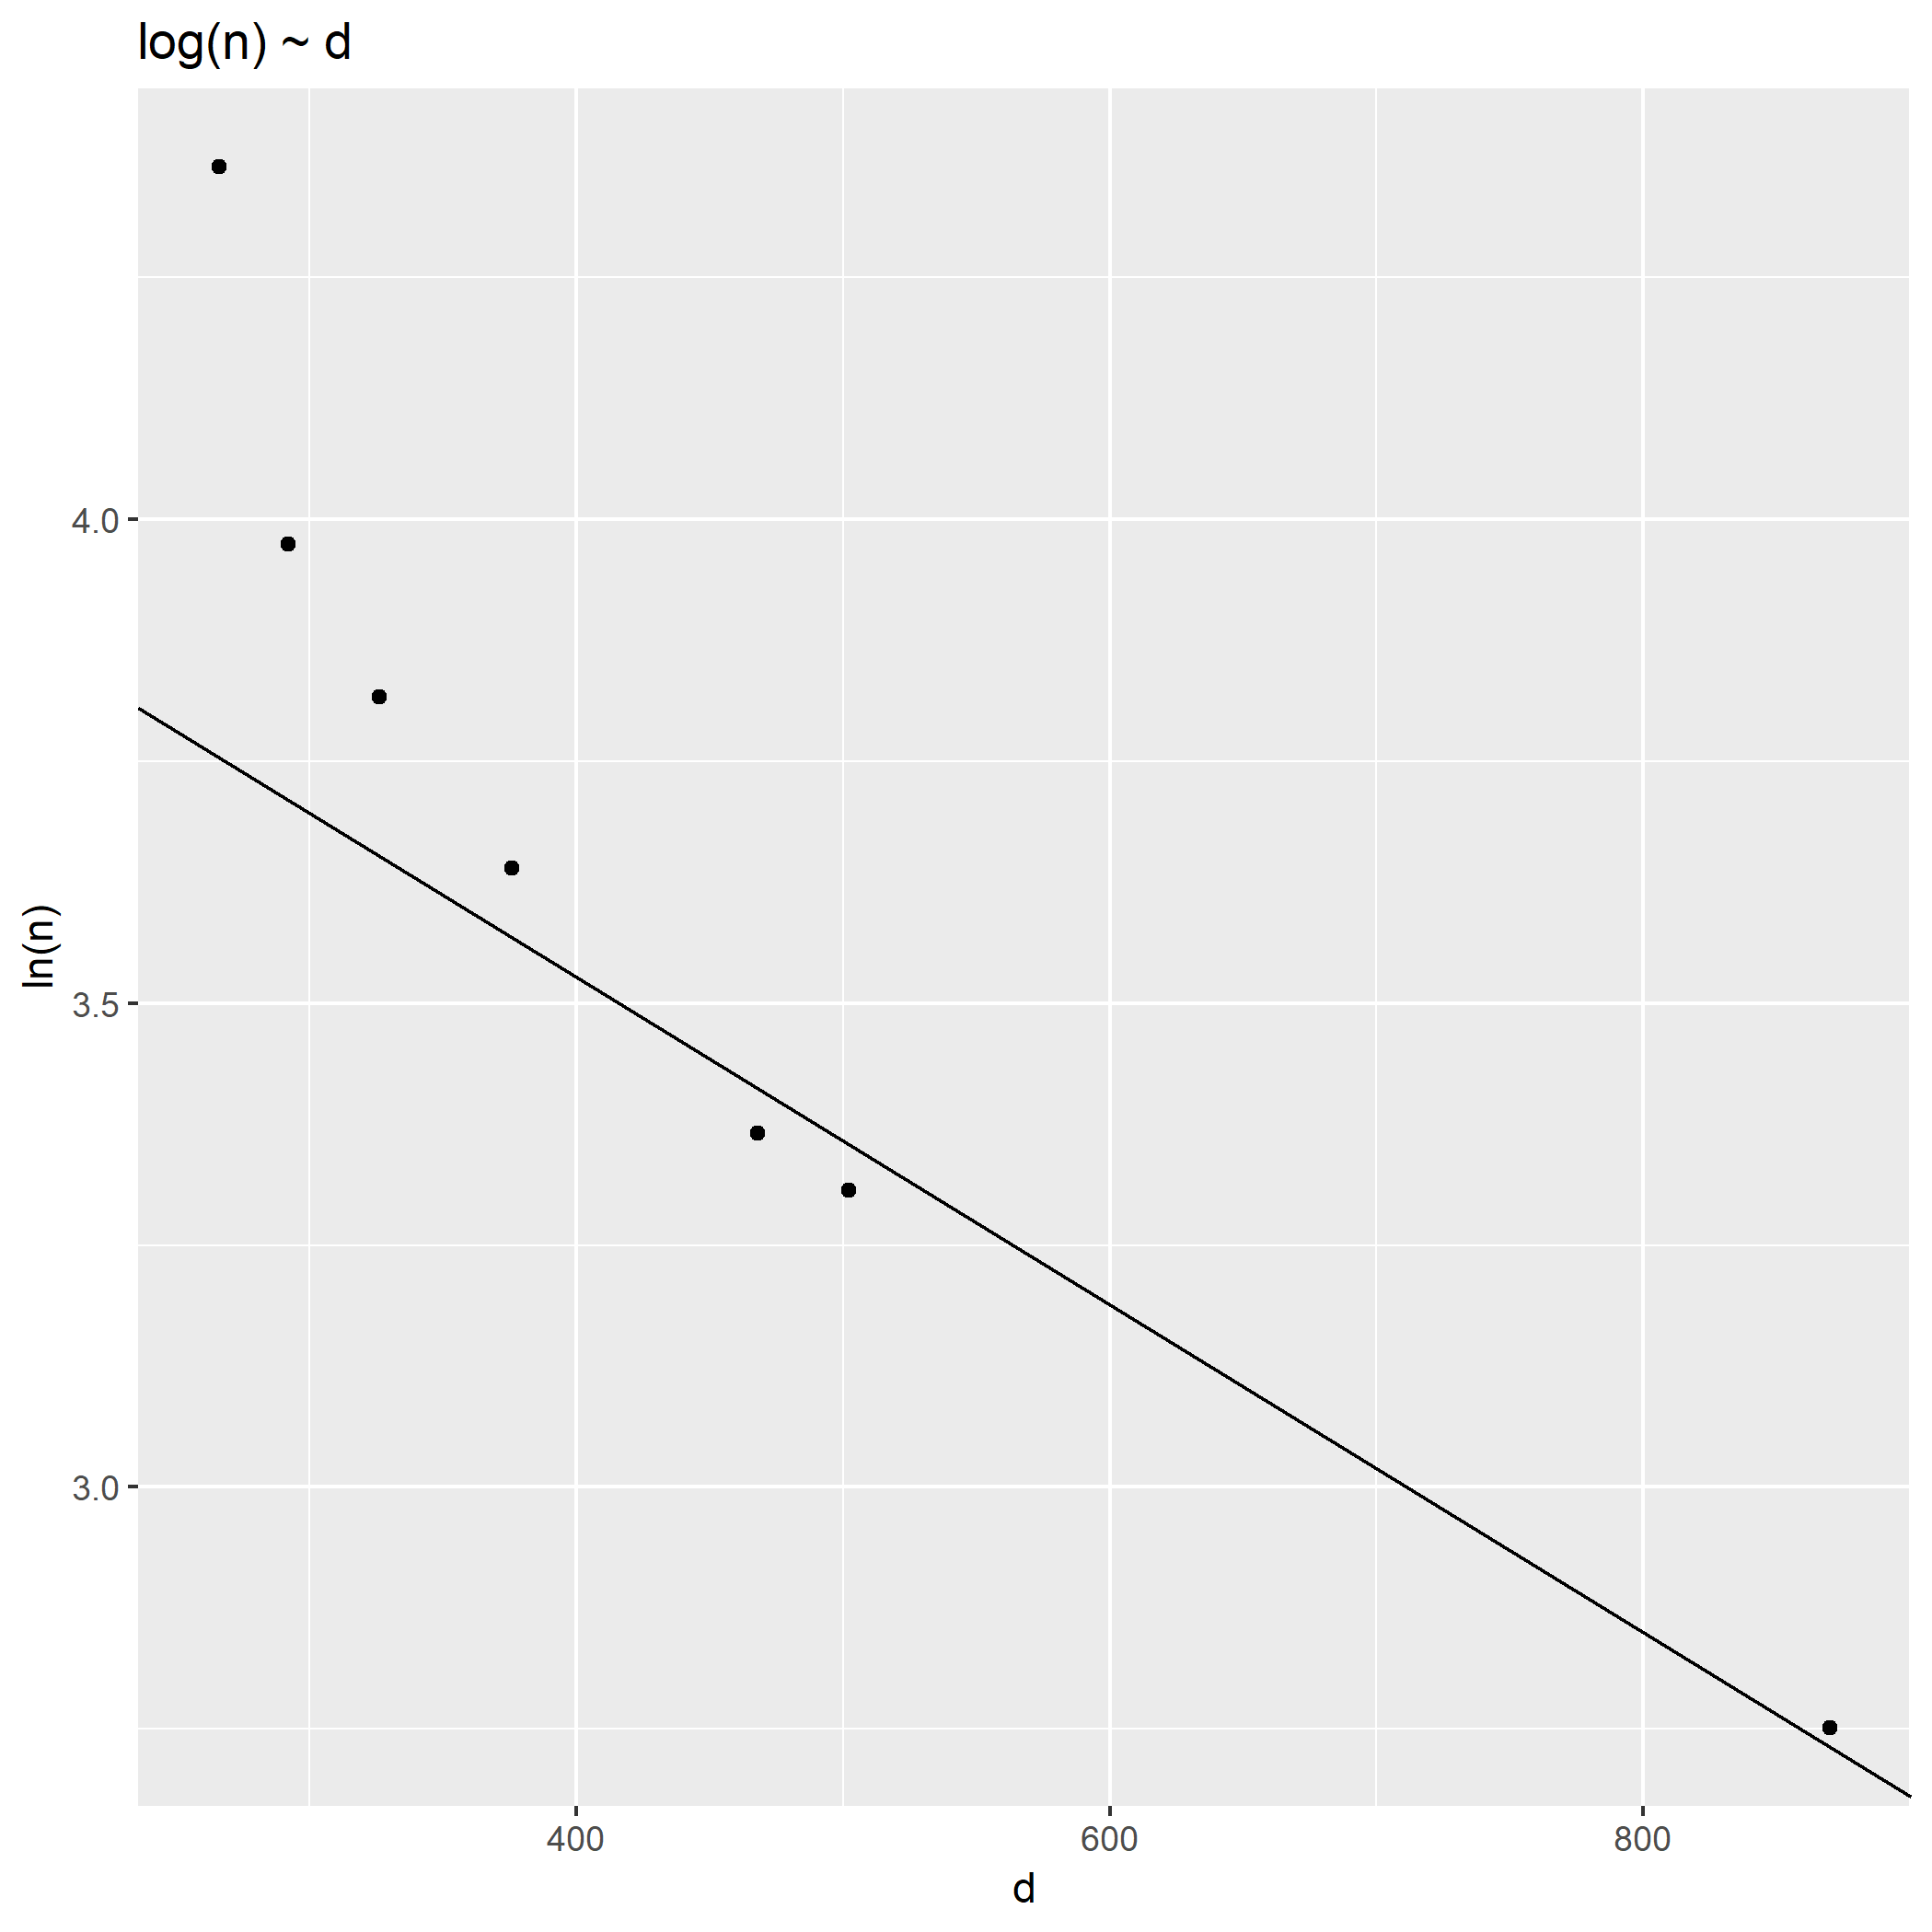
\includegraphics[width = 0.4\textwidth]{../Data/raw_points_line.png}
                \caption{Standard Curve with Fitting Line}
                \label{raw.curve.line}
            \end{figure}
            
        \subsection{pBR322 Digestion Data}
            The distance of every well is shown below, using pixel unit.
            \begin{table}[H]
                \caption{Distance}
                \centering
                \begin{tabular}{|l|c|c|c|c|c|c|c|}
                    \hline
                    Tube&E&H&P&EH&EP&HP&EHP\\
                    \hline
                    Distance&400.125&418.12&388.082&424.118&472.004&520.004&530.015\\
                    (pixels)&&682.237&&676.027&486.037&596.03&602.003\\
                    &&&&830.039&&668.012&830.002\\
                    &&&&924.078&&&928.002\\
                    \hline
                \end{tabular}
                \label{data.table}
            \end{table}
            So using the equation derived above, we can get the estimated sequence length (rounded to integer),
            \begin{table}[H]
                \caption{Length}
                \centering
                \begin{tabular}{|l|c|c|c|c|c|c|c|}
                    \hline
                    Tube&E&H&P&EH&EP&HP&EHP\\
                    \hline
                    Length&3342&3112&3499&3041&2523&2089&2009\\
                    (bps)&&1107&&1135&2388&1552&1517\\
                    &&&&621&&1169&621\\
                    &&&&430&&&423\\
                    \hline
                \end{tabular}
                \label{data.len.table}
            \end{table}
            and also the logarithm of length,
            \begin{table}[H]
                \caption{Logarithm of Length}
                \centering
                \begin{tabular}{|l|c|c|c|c|c|c|c|}
                    \hline
                    Tube&E&H&P&EH&EP&HP&EHP\\
                    \hline
                    log(Length)&3.524&3.493&3.544&3.483&3.402&3.32&3.303\\
                    &&3.044&&3.055&3.378&3.191&3.181\\
                    &&&&2.793&&3.068&2.793\\
                    &&&&2.633&&&2.626\\
                    \hline
                \end{tabular}
                \label{data.log.table}
            \end{table}
        \subsection{pBR322 Mapping}
            \begin{figure}[H]
                \centering
                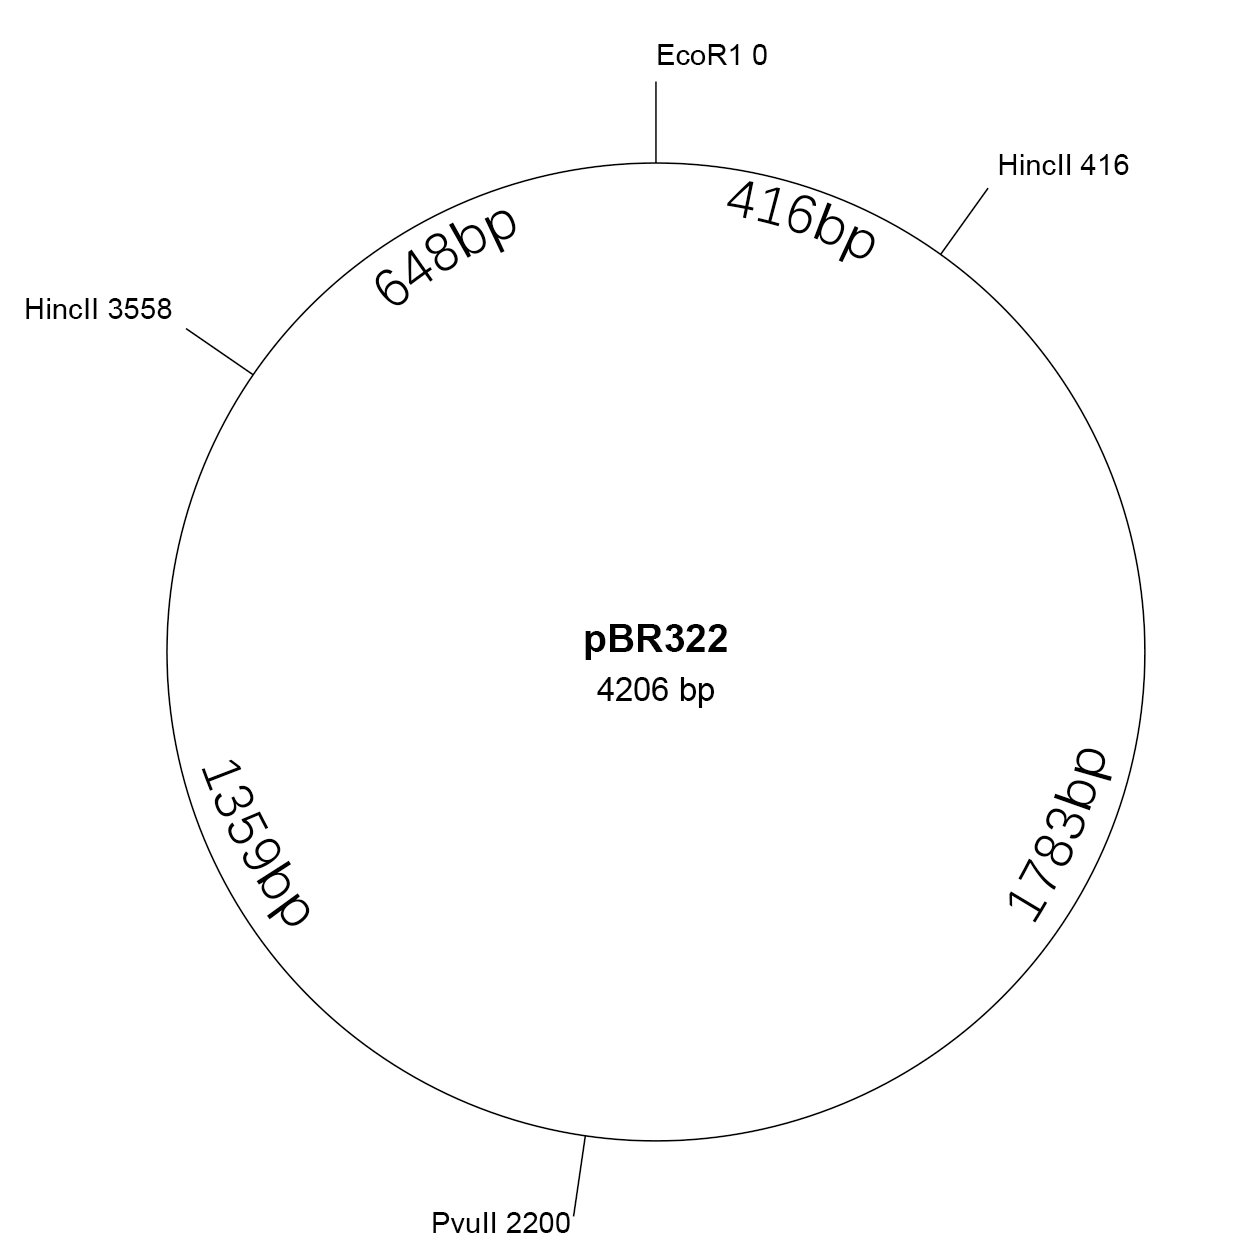
\includegraphics[width = 0.4\linewidth]{../Data/Plasmid/final.png}
                \caption{Mapping Result}
                \label{final.map}
            \end{figure}
    
    \section{Discussion}
        \subsection{Standard Curve}
            First, I tried to discard the points with larger length, which is out of the gel's resolving ability. The lines are derived from linear regression, namely, least squared method (calculation not shown).
            \begin{figure}[H]
                \begin{minipage}[t]{0.5\textwidth}
                    \centering
                    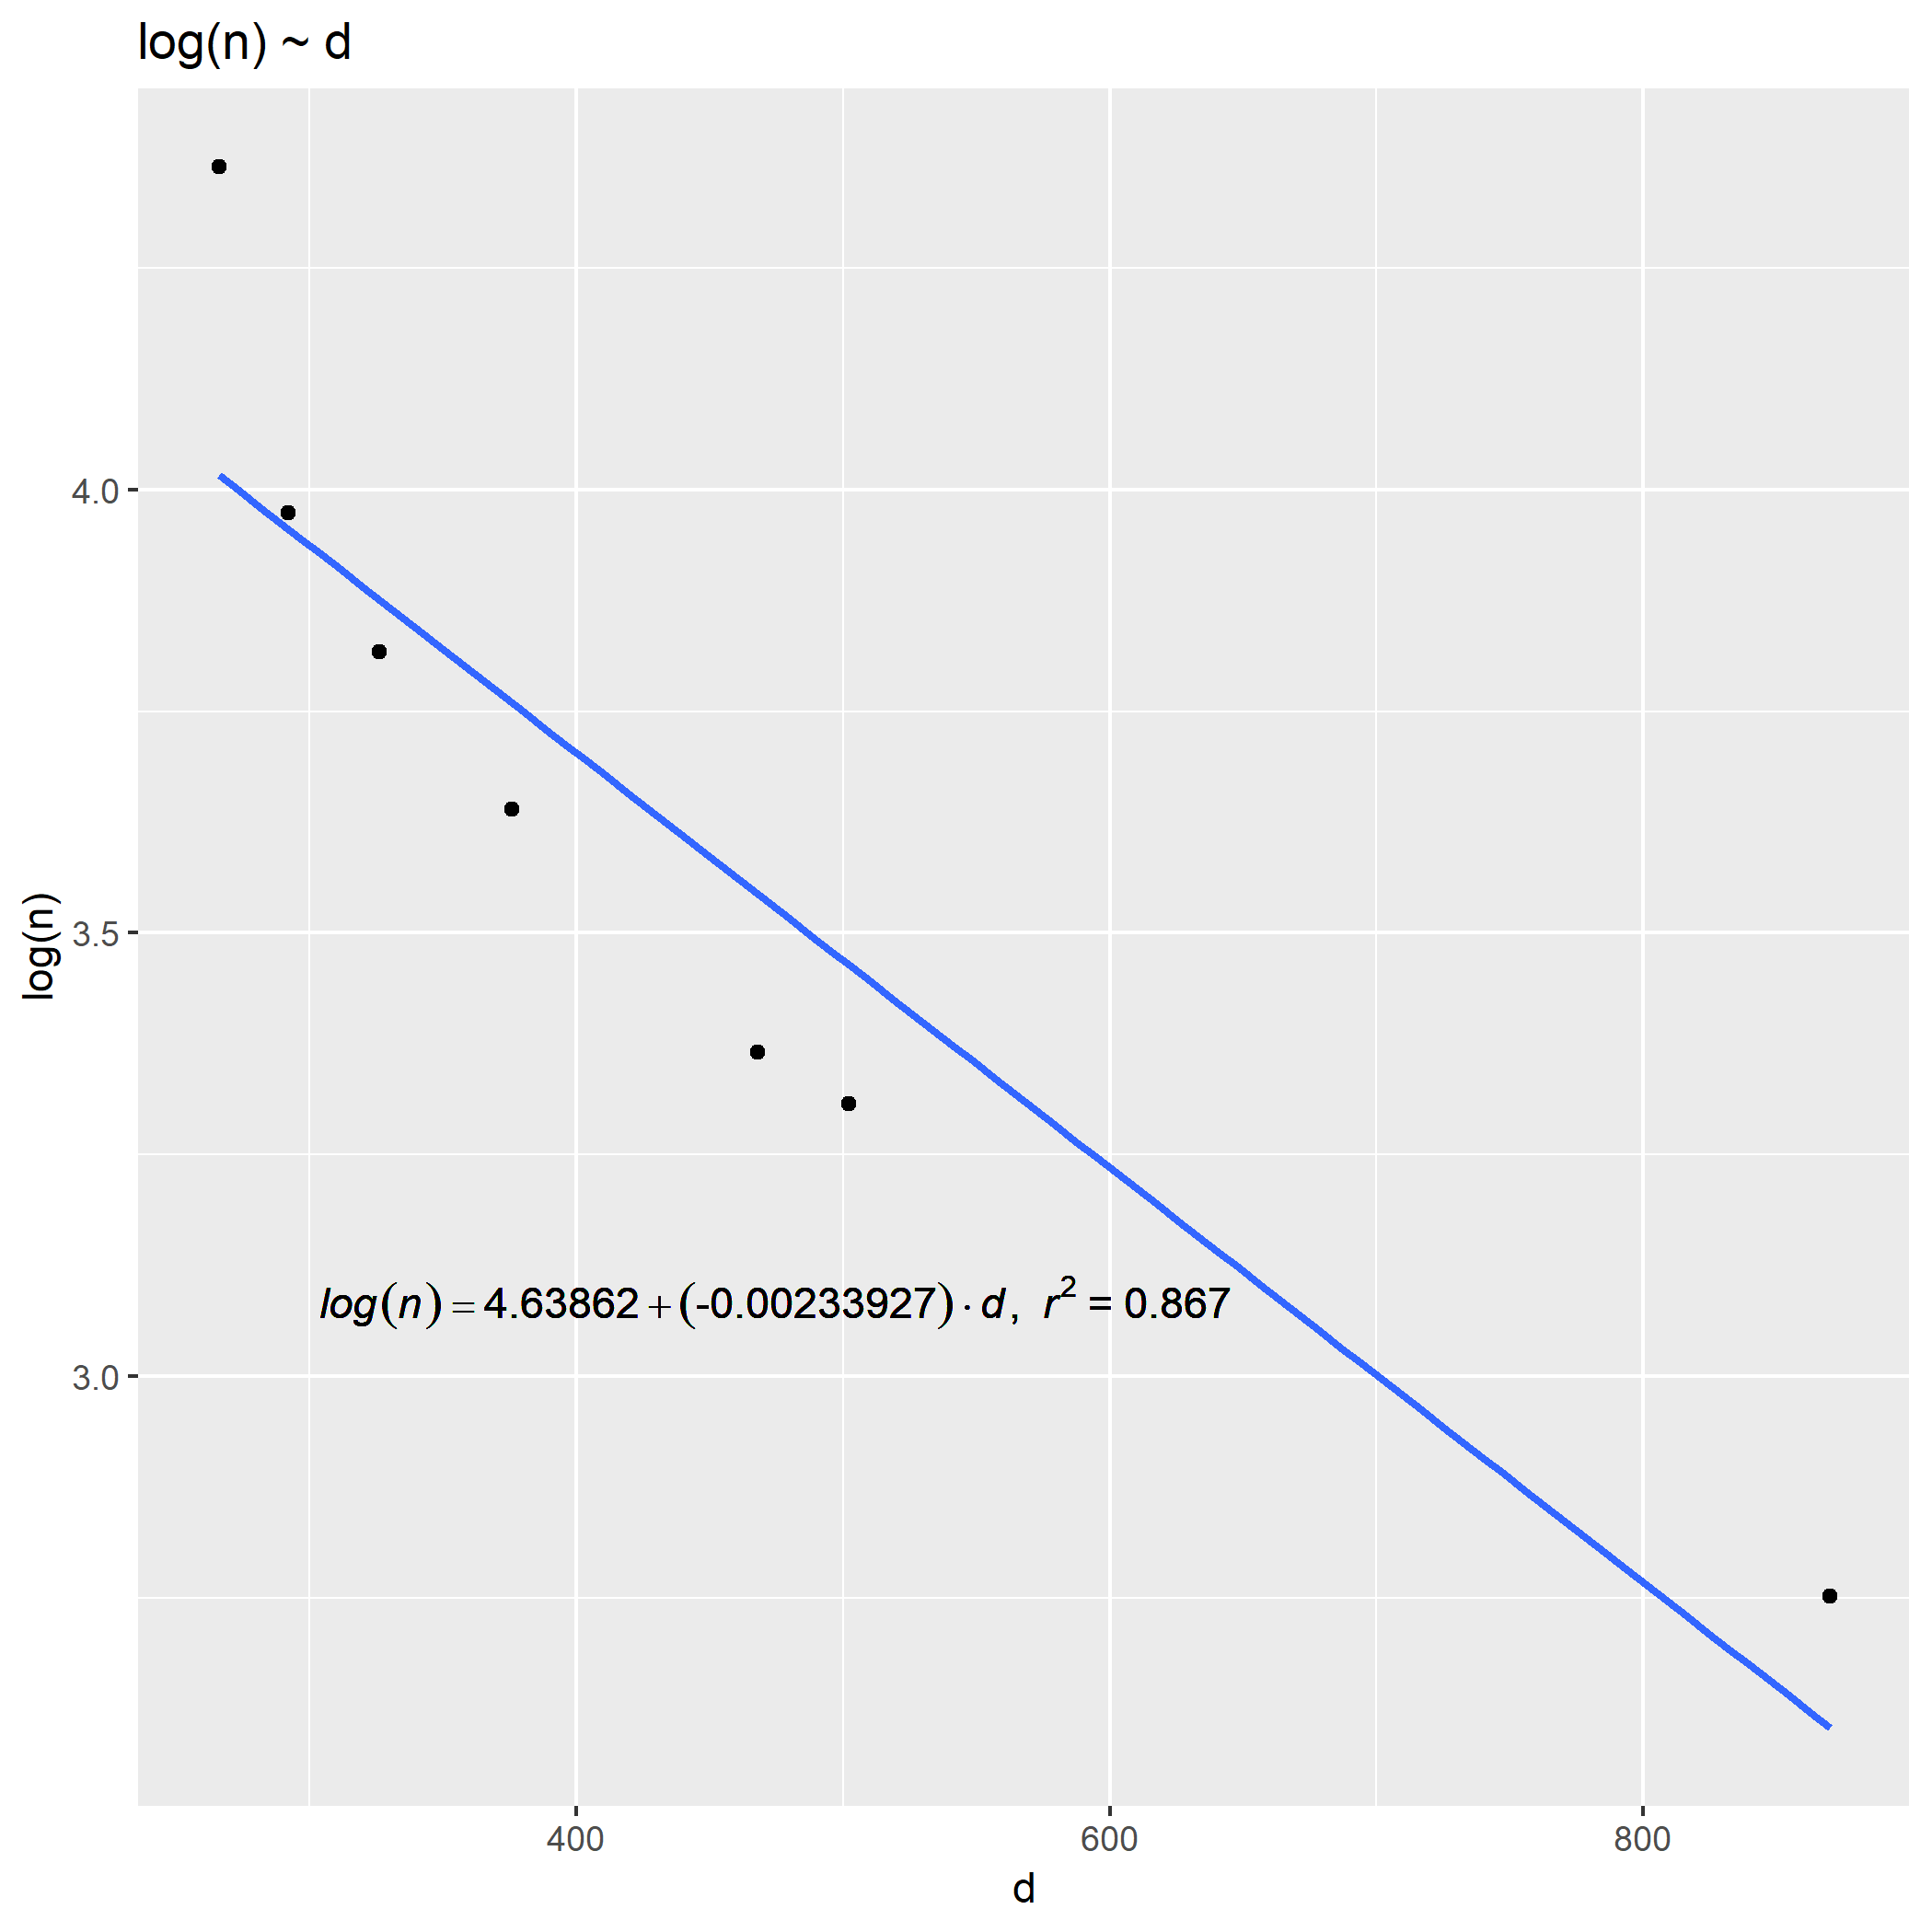
\includegraphics[width = 0.8\linewidth]{../Data/discard_1.png}
                    \caption{No Discarding}
                    \label{dis.0}
                \end{minipage}
                \begin{minipage}[t]{0.5\textwidth}
                    \centering
                    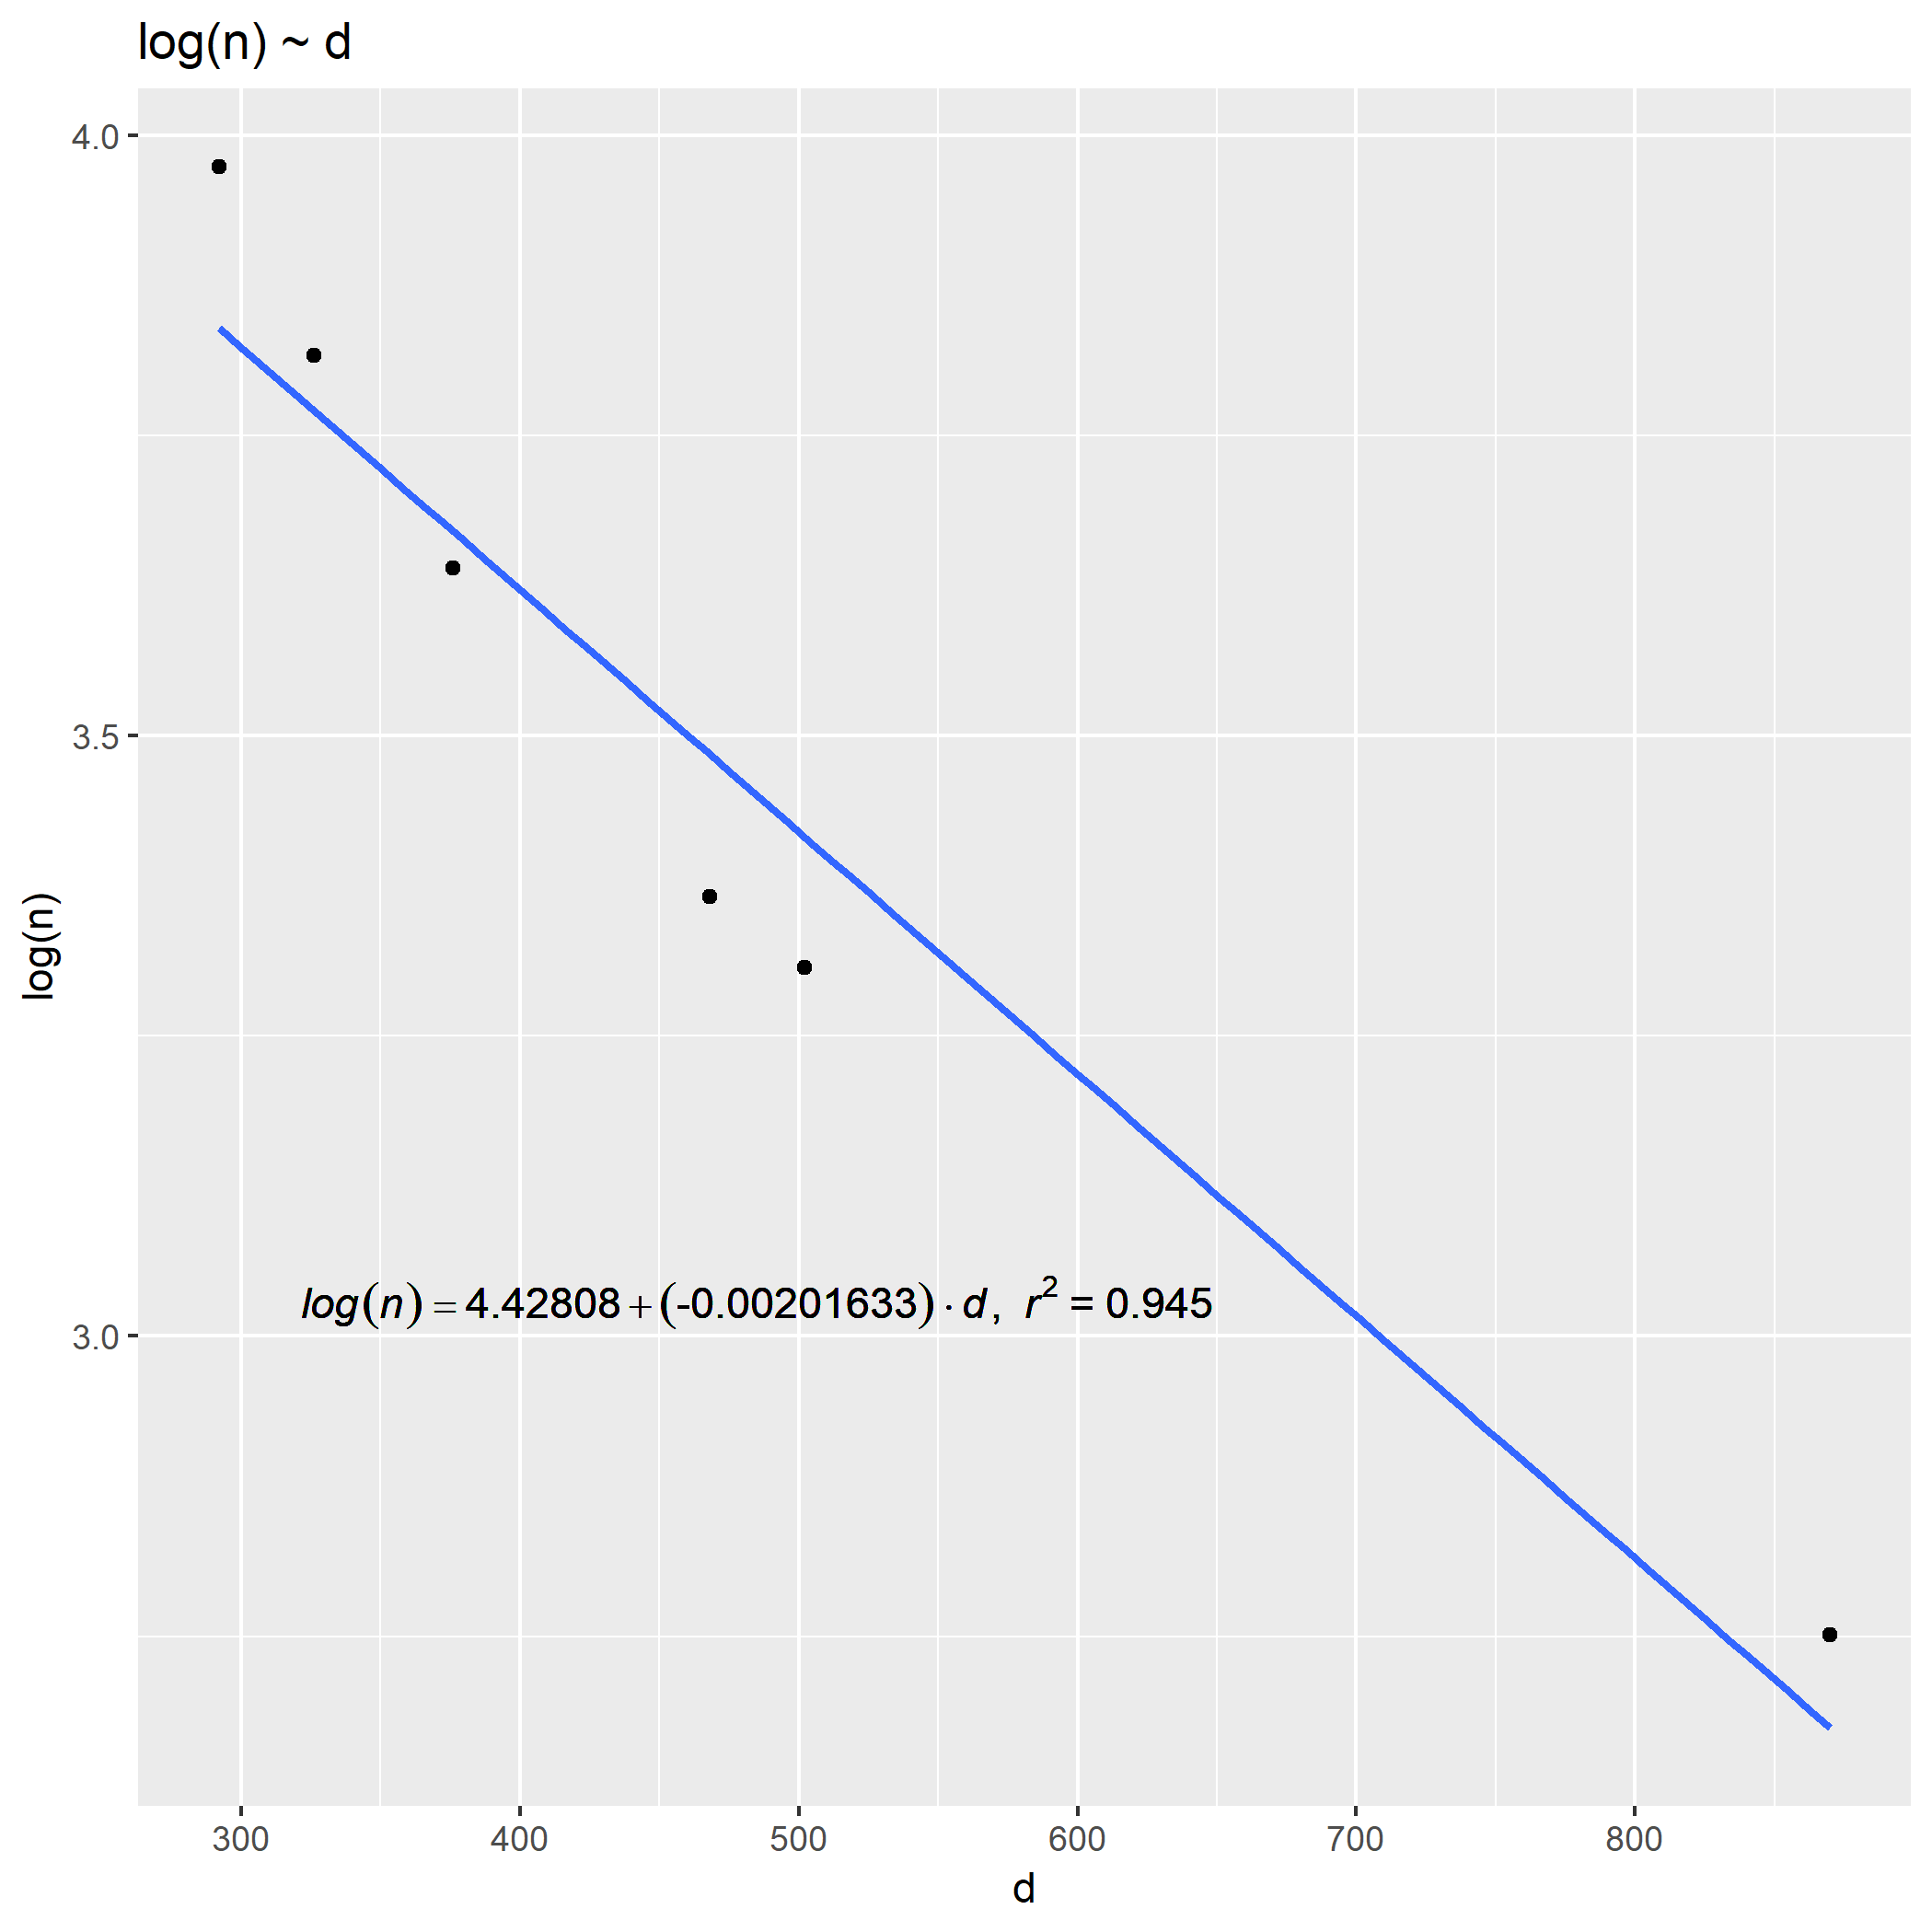
\includegraphics[width = 0.8\linewidth]{../Data/discard_2.png}
                    \caption{Discarding Point 1}
                    \label{dis.1}
                \end{minipage}
            \end{figure}
            \begin{figure}[H]
                \begin{minipage}[t]{0.5\textwidth}
                    \centering
                    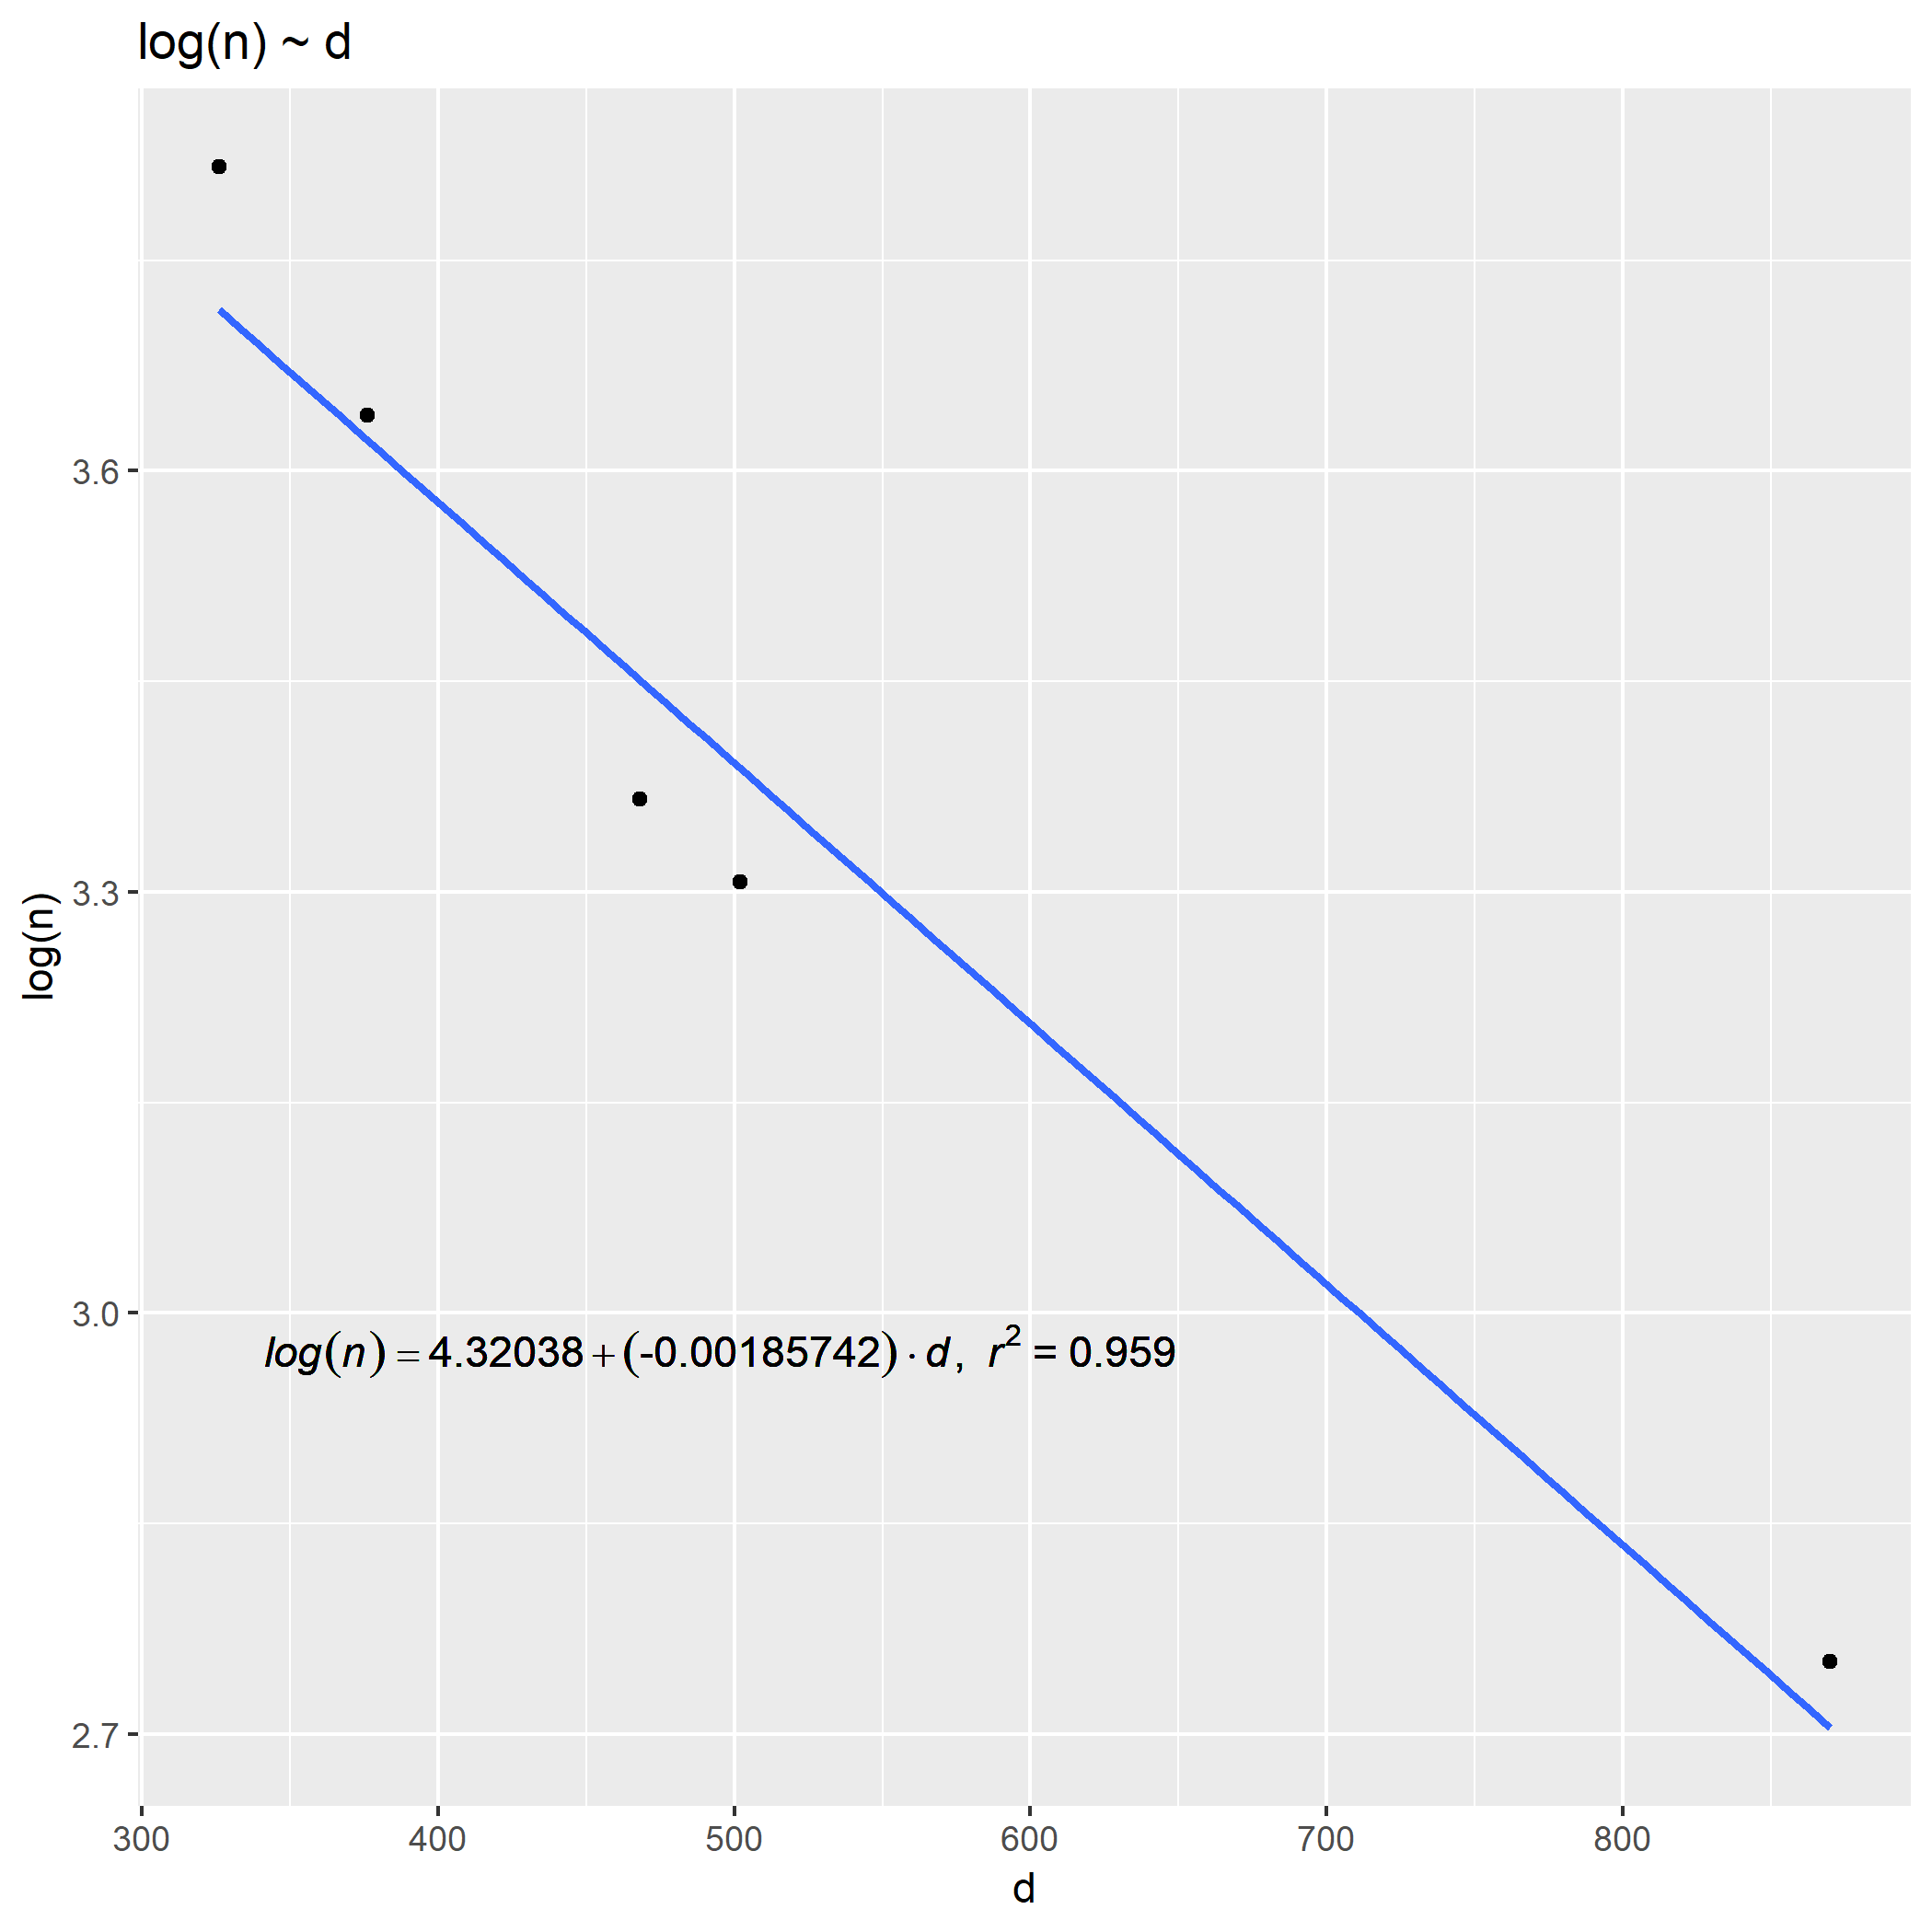
\includegraphics[width = 0.8\linewidth]{../Data/discard_3.png}
                    \caption{Discarding Point 1$\sim$2}
                    \label{dis.2}
                \end{minipage}
                \begin{minipage}[t]{0.5\textwidth}
                    \centering
                    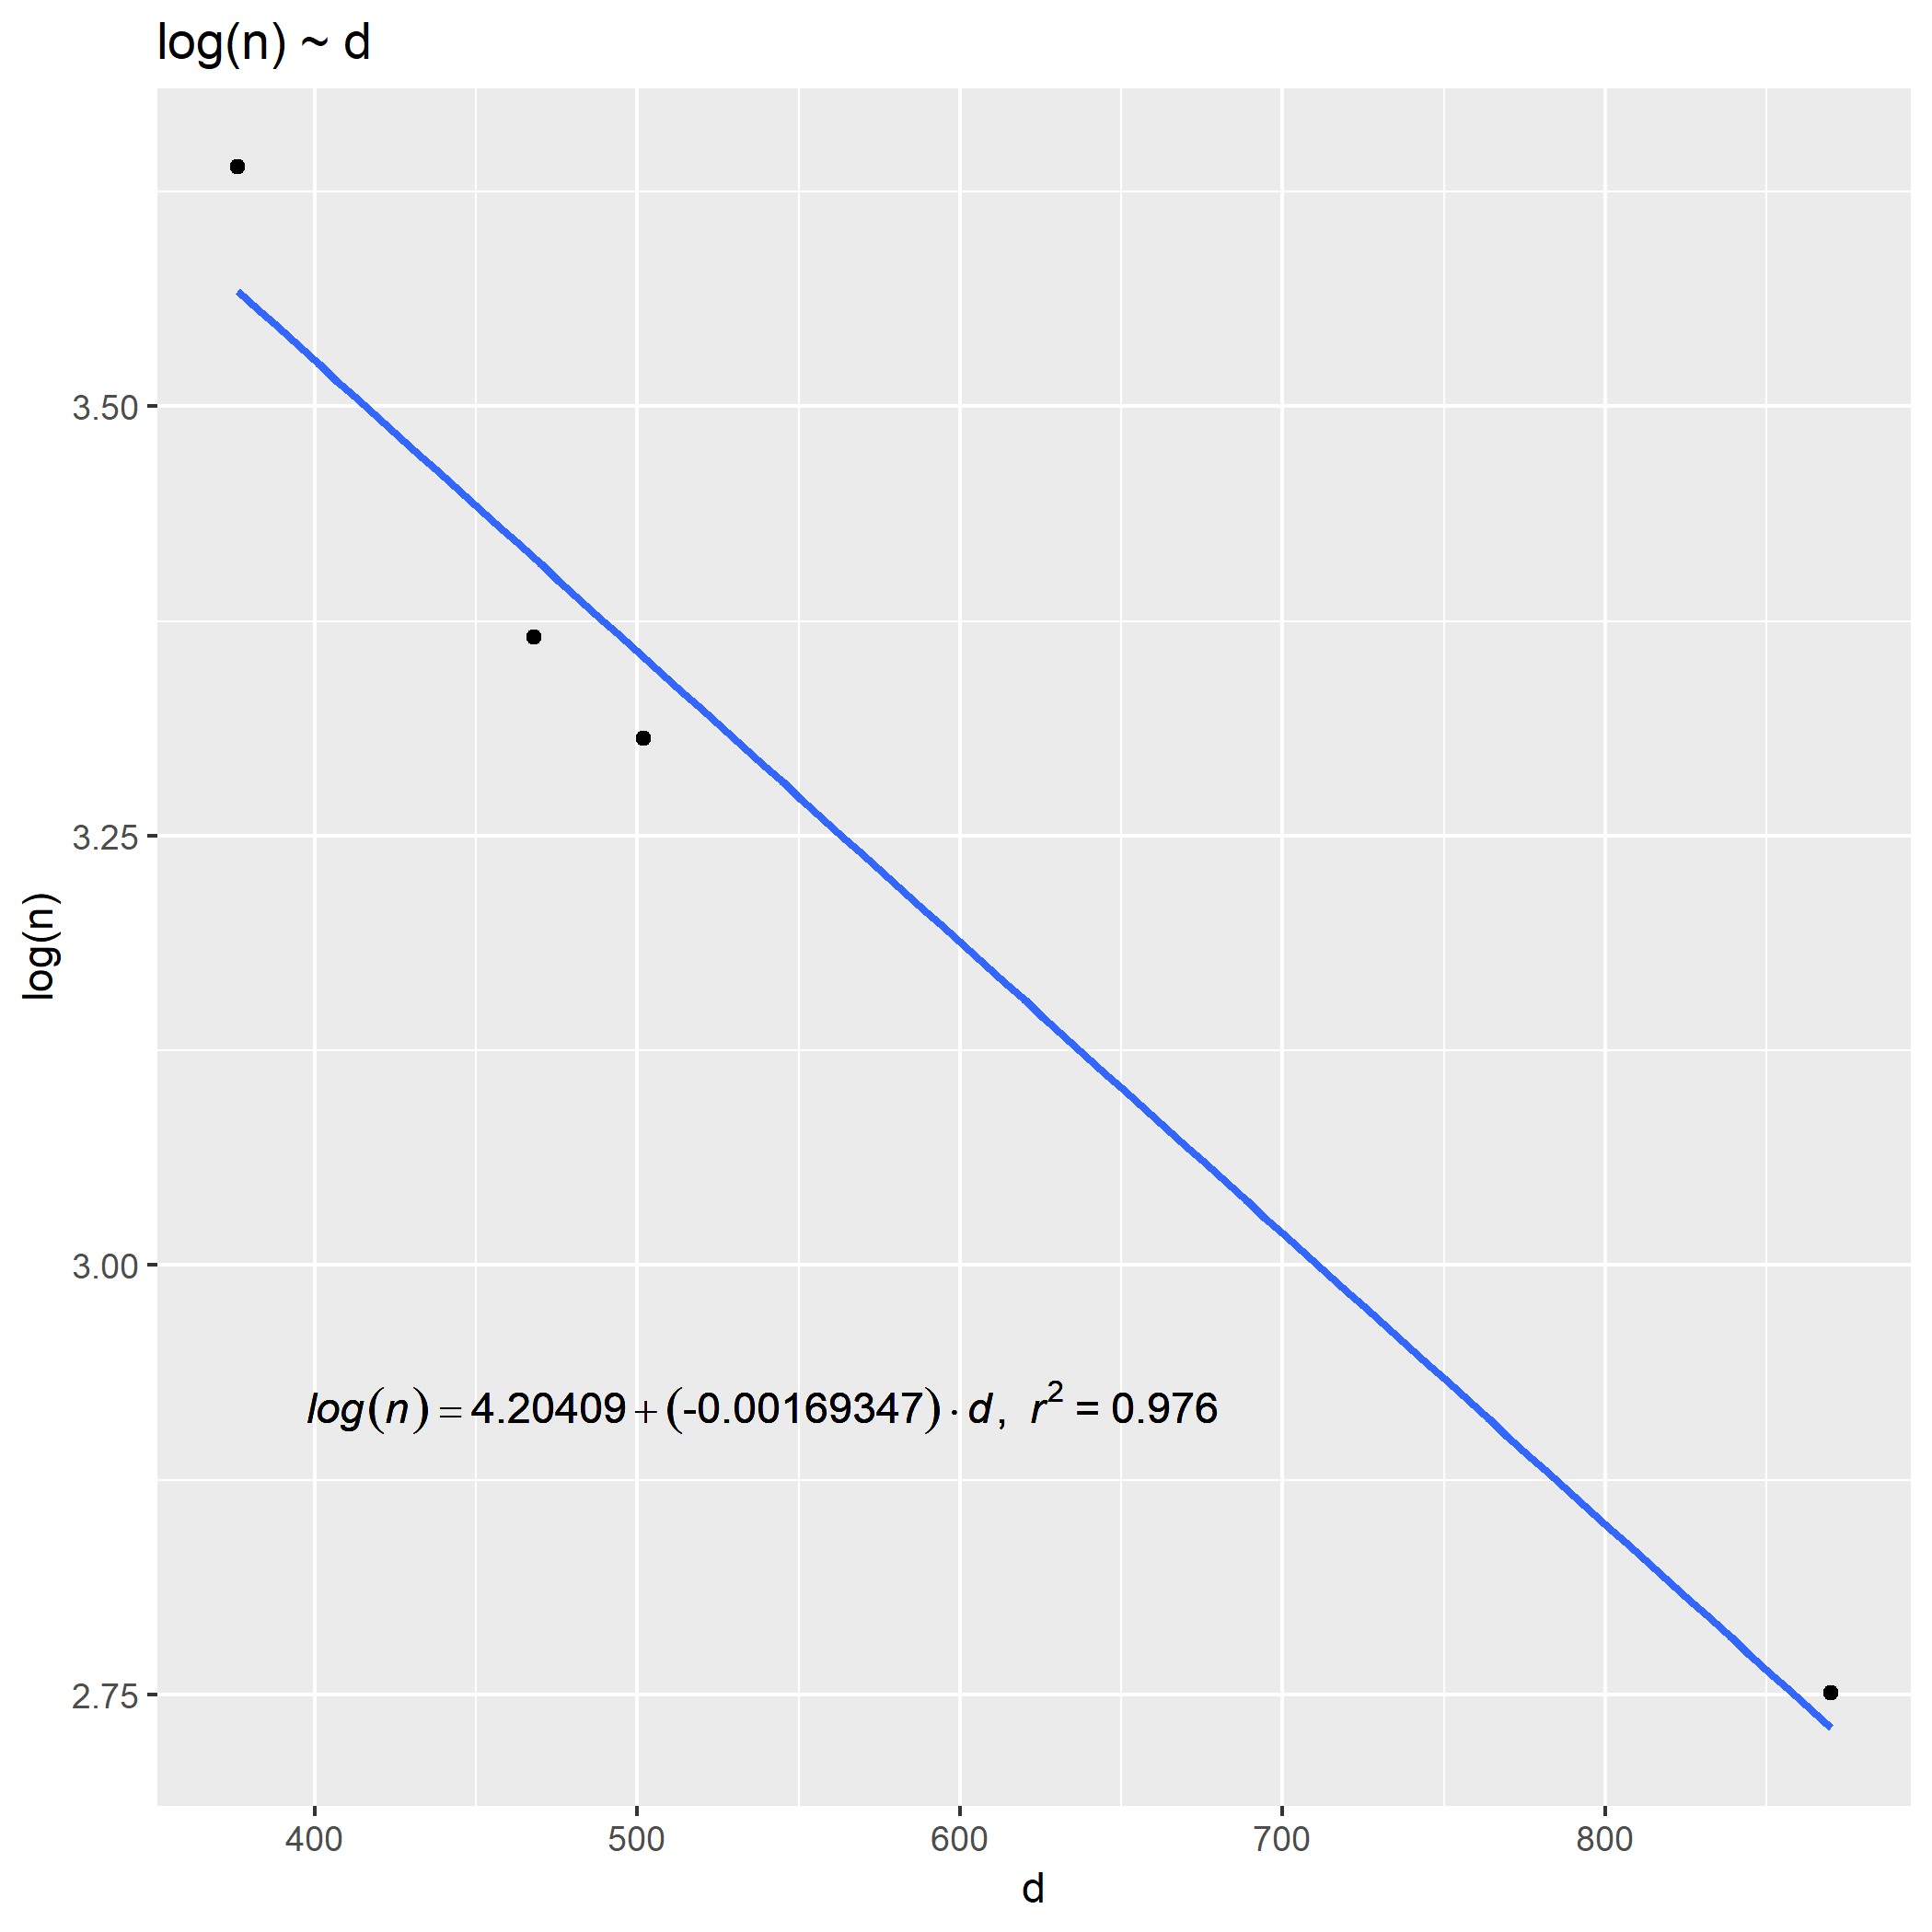
\includegraphics[width = 0.8\linewidth]{../Data/discard_4.png}
                    \caption{Discarding Point 1$\sim$3}
                    \label{dis.3}
                \end{minipage}
            \end{figure}

            Then compared the $R^2$, we can see that discarding first 3 points leads to the highest $R^2$ as $0.976$. In addition, these three points are also longer than 5000bp, larger than the ability of gel resolution. 

            If we discard more points, we would get higher $R^2$, but we will lose data information and increase the effect of random error.

            Finally we will use Figure \ref{dis.3} as the fitting line, which has already been plotted in Figure \ref{raw.curve.line} in \textbf{Result} part.

            In conclusion,
            $$
            \begin{aligned}
                \text{log}(n) &= 4.2 - 1.7\times 10 ^ {-3} \cdot d\\
                n &= exp(4.2 - 1.7 \times 10 ^ {-3} \cdot d)
            \end{aligned}
            $$

        \subsection{Relative Position Analysis}
            For convenience, I label bands from tube \textbf{E, H, P, EH, EP, HP, EHP}.
            \begin{figure}[H]
                \centering
                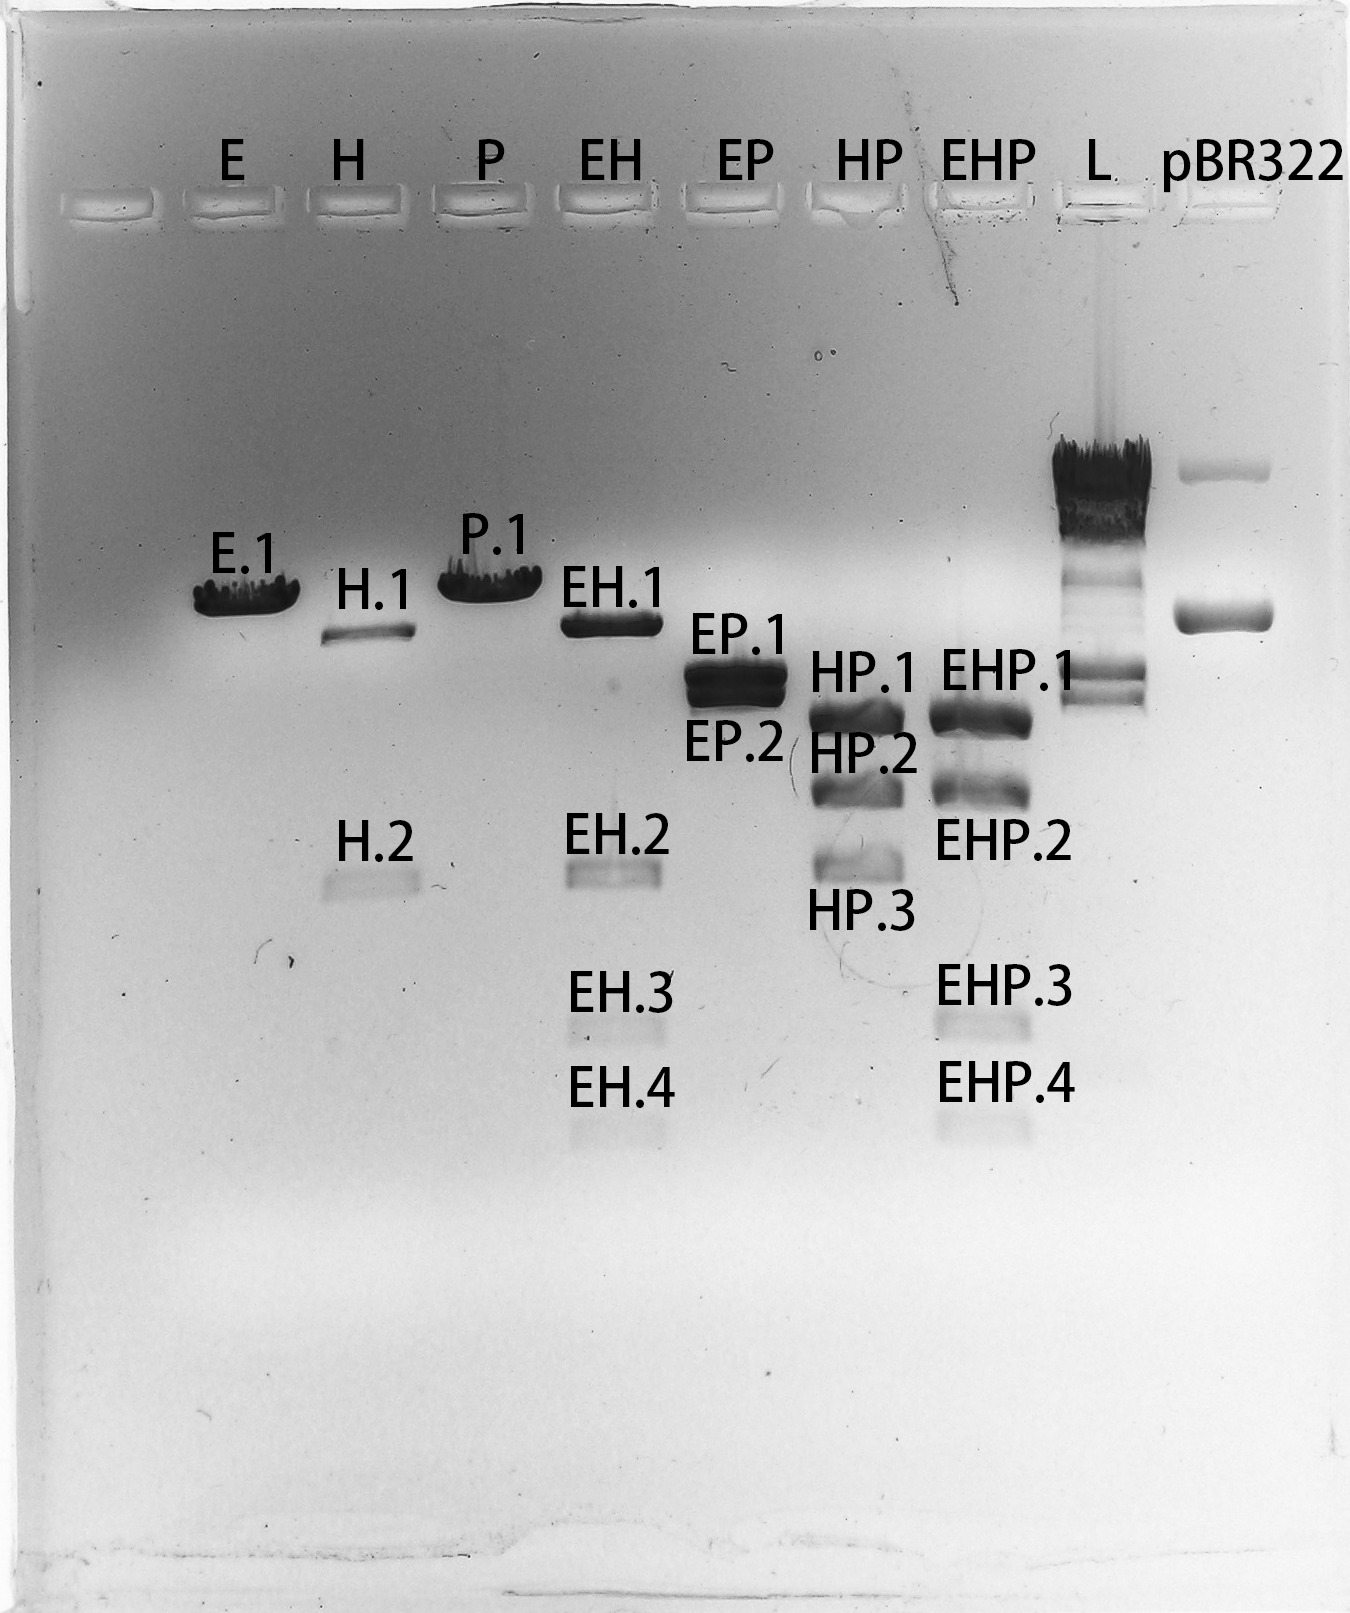
\includegraphics[width = 0.4\linewidth]{../Data/xun_and_sam_label.png}
                \caption{Labeled Bands}
                \label{label.bands}
            \end{figure}
            \subsubsection{Single Enzyme Digestion}
                For tube \textbf{E, H, P}, we can see that \textbf{E, P} have two similar single bands, but \textbf{H} has two bands, which indicates that enzyme EcoR1 and PvuII cut the plasmid at one site, while HincII cuts at two sites. The picture below demonstrates this more clearly.
                \begin{figure}[H]
                    \centering
                    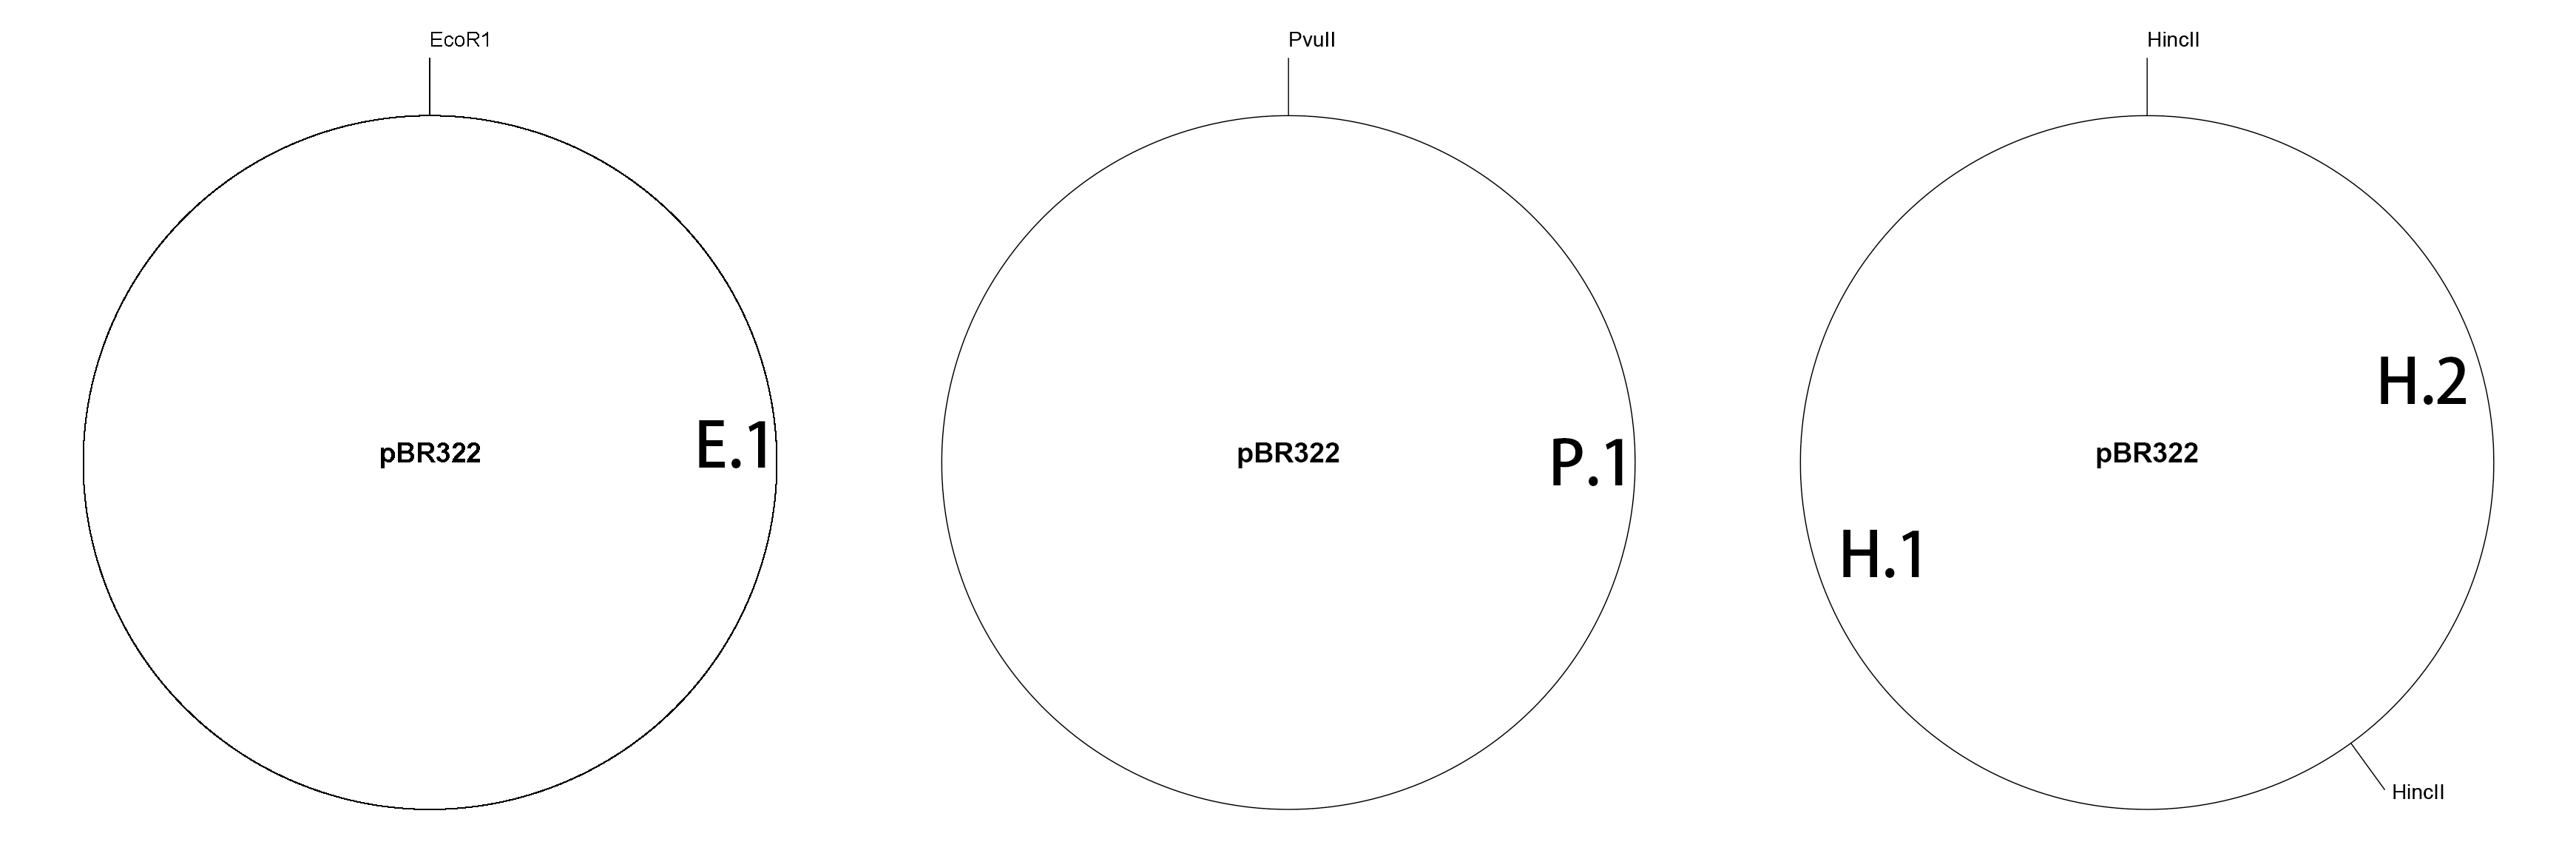
\includegraphics[width = 0.9\linewidth]{../Data/Plasmid/single.png}
                    \caption{Number of Cutting Sites}
                    \label{single.cut}
                \end{figure}
                Here, I choose different lengths for H.1 and H.2, because their bands' distances are different, causing H.1 to be longer with small distance, and H.2 to be shorter.
                $$\text{pBR322}\underset{\text{HincII}}{\rightarrow}\text{H.1} + \text{H.2}$$
                $$\text{H.1} > \text{H.2}$$

            \subsubsection{Two Enzymes Digestion}
                After we get the number of cutting sites of three enzymes, we can analysis their combination digestion.

                \paragraph{\textbf{EH} tube} There are 4 different bands, and two of them (EH.1, EH.2) are almost the same as bands of \textbf{H}'s (H.1, H.2). However, as it is digested by EcoR1 and HincII, who have 1 and 2 cutting sites. So there should be 3 sites, and 3 bands. That is, HincII cuts the plasmid into two part, and EcoR1 cuts one of these two in to another two parts. Considering two same bands as \textbf{H}'s, the reaction of EcoR1's cutting is not complete, remaining small amount of HincII's product. In addition, as the signal of EH.1 is stronger than EH.2's, it is very likely that EH.2 (also H.2) should be cut into EH.3 and EH.4 but reaction is not complete, which means EcoR1's site might be located on EH.2 (also H.2), namely, shorter part between two HincII sites.
                $$\text{H.2} \underset{\text{EcoR1}}{\rightarrow}\text{EH.3} + \text{EH.4}\text{ (highly likely)}$$

                \paragraph{\textbf{EP} tube} The phenomenon is similar to \textbf{H}'s. Simply put, EcoR1's and PvuII's cutting sites lead to two fragments with different but similar lengths, since their distances are similar. So, EcoR1's cutting site should be about the opposite of PvuII's site.
                $$\text{pBR322}\underset{\text{EcoR1, PvuII}}{\rightarrow}\text{EP.1}+\text{EP.2} \text{ (similar length)}$$

                \paragraph{\textbf{HP} tube} This can be analyzed as \textbf{EH} tube, but with better and clearer result. The digestion process can be explained as follows\footnote{There is no order of two enzyme reactions, but explaining them in order can make reaction process clear.}. HincII cuts plasmid into H.1 and H.2. Then, PvuII cuts H.1 into HP.1 and HP.2, leaving H.2 as HP.3, for their lengths are similar. So, PvuII's cutting site is located in H.1, namely, the longer part between two hincII sites.
                $$\text{H.1}\underset{\text{PvuII}}{\rightarrow}\text{HP.1} + \text{HP.2}$$

                \paragraph{Two Enzymes Conclusion} We have got three conclusions:
                    \begin{enumerate}
                        \item EcoR1 is on shorter part between HincII. (Assumption with high likelihood)
                        \item EcoR1 is about the opposite of PvuII.
                        \item PvuII is on longer part between HincII.
                    \end{enumerate}
                In addition, it is mentioned above that EH.3/EH.4 are products of H.1 or H.2. And HP.1/HP.2 are products of H.1. However, both EH.3 and EH.4 is shorter than HP.1 and HP.2, for their smaller distances, which indicates that if we connect EH.3 with EH.4, the summation of length is less than HP.1 plus HP.2. That is, EH.3/EH.4 and HP.1/HP.2 come from two different reagents, EH.3/EH.4 from shorter one (H.2), and HP.1/HP.2 from longer one (H.1). So, here is the map.
                \begin{figure}[H]
                    \centering
                    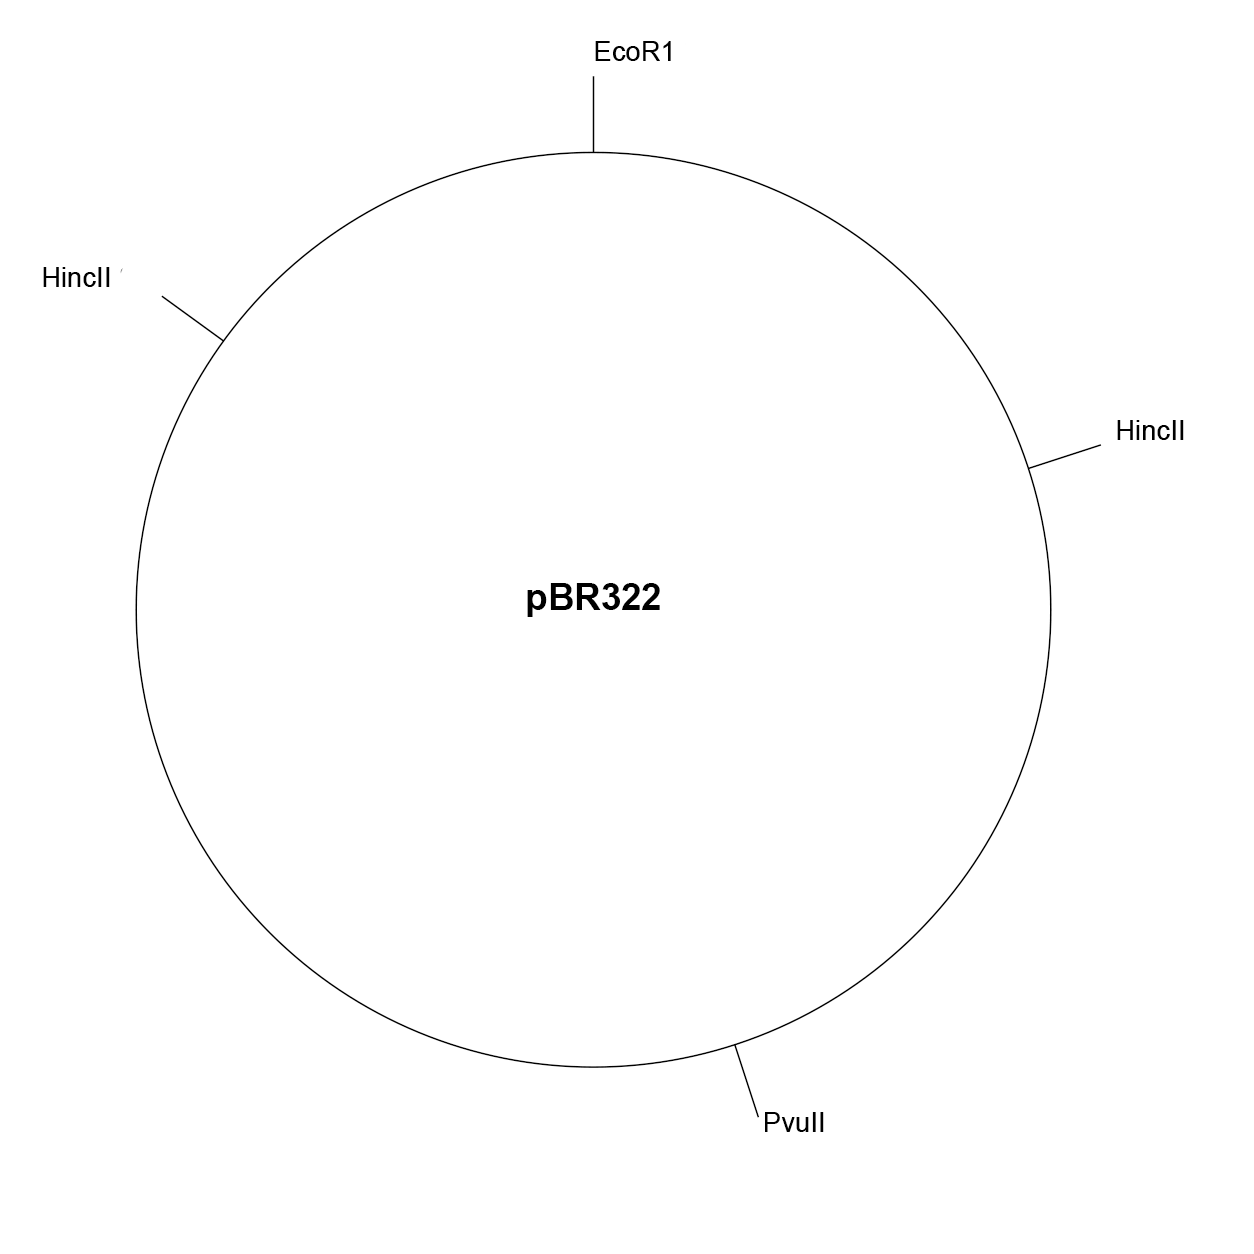
\includegraphics[width = 0.4\linewidth]{../Data/Plasmid/III.png}
                    \caption{Possible Map}
                    \label{possible.map}
                \end{figure}

            \subsubsection{Three Enzyme Digestion}
                For \textbf{EHP} tube, EHP.1 and EHP.2 are similar with HP.1 and HP.2. Meanwhile, EHP.3 and EHP.4 are similar with EH.3 and EH.4.

                The bands correspond with the mapping result\footnote{No fixed order in real reaction.}:
                $$\begin{aligned}
                \text{pBR322}&\underset{\text{HincII}}{\rightarrow}&\text{H.1} &+ \text{H.2}\\
                \text{H.1}&\underset{\text{PvuII}}{\rightarrow}&\text{EHP.1} &+ \text{EHP.2}\\
                \text{H.2}&\underset{\text{EcoR1}}{\rightarrow}&\text{EHP.3} &+ \text{EHP.4}\\
                \end{aligned}$$

        \subsection{Data Analysis}
            Before we start to calculate the length, we have to clean the raw length data (Table \ref{data.len.table} and Table \ref{data.log.table}). As we have known that some bands have equal length, some are the summation of other bands, and some bands equal to the whole plasmid.

            First, we will estimate the total length of plasmid by calculating the average of 7 summations.
            \begin{table}[H]
                \centering
                \caption{Total Length of Each Well}
                \begin{threeparttable}
                    \begin{tabular}{|l|c|c|c|c|c|c|c|}
                        \hline
                        Tube&E&H&P&EH&EP&HP&EHP\\
                        \hline
                        Length&3342&3112&3499&3041&2523&2089&2009\\
                        (bps)&&1107&&(1135)&2388&1552&1517\\
                        &&&&621&&1169&621\\
                        &&&&430&&&423\\
                        \hline
                        total&3342&4219&3499&4092\tnote{*}&4911&4810&4570\\
                        \hline
                        average&\multicolumn{7}{|c|}{4206}\\
                        \hline
                    \end{tabular}
                    \begin{tablenotes}
                        \footnotesize
                        \item[*] EH.2 (length = 1135) is remaining of incomplete reaction, not included.
                    \end{tablenotes}
                \end{threeparttable}
                \label{data.len.table.total}
            \end{table}

            So, the estimated total length is 4206bp. Assuming the total length is true, we can standardize all the lengths to their ratio to total length.

            $$\text{Ratio} = \frac{\text{Length}}{\text{Total Length}} \in [0, 1]$$

            Then the data will become:
            \begin{table}[H]
                \caption{Ratio of All Fragments}
                \centering
                \begin{tabular}{|l|c|c|c|c|c|c|c|}
                    \hline
                    Tube&E&H&P&EH&EP&HP&EHP\\
                    \hline
                    Ratio&1&0.738&1&0.743&0.514&0.434&0.44\\
                    &&0.262&&(0.27)&0.486&0.323&0.332\\
                    &&&&0.152&&0.243&0.136\\
                    &&&&0.105&&&0.092\\
                    \hline
                \end{tabular}
                \label{data.ratio}
            \end{table}

            Then we will use a mathematical method solving equations to get the most probable result.

            Since EHP.1/EHP.2/EHP.3/EHP.4 are 4 indivisible fragments and others are made from them, we assume their true ratio are $x_1, x_2, x_3, x_4$, where $x_1 + x_2 + x_3 + x_4 = 1$.

            Thus, the assumption is,
            \begin{table}[H]
                \caption{Ratio of All Fragments}
                \centering
                \begin{threeparttable}
                    \begin{tabular}{|l|c|c|c|c|c|c|c|}
                        \hline
                        Tube&E&H&P&EH&EP&HP&EHP\\
                        \hline
                        Ratio&1&$x_1 + x_2$&1&$x_1 + x_2$&$\text{ - }^*$&$x_1$&$x_1$\\
                        &&$x_3 + x_4$&&$(x_3 + x_4)$&$\text{ - }^*$&$x_2$&$x_2$\\
                        &&&&$x_3$&&$x_3 + x_4$&$x_3$\\
                        &&&&$x_4$&&&$x_4$\\
                        \hline
                    \end{tabular}
                    \begin{tablenotes}
                            \footnotesize
                            \item[*] EP.1/EP.2's composition is unknown.
                        \end{tablenotes}
                \end{threeparttable}
                \label{data.ratio.x}
            \end{table}

            So, for all fragments, there are assumption ratio and experimental ratio. We can calculate the error by squared error:
            $$\text{Error} = (\text{Ratio} - \text{Ratio}_{\text{Experi}})^2$$

            Then, we can choose $x_1, x_2, x_3, x_4$ to minimize the error. The total error is calculated as:
            $$\begin{aligned}
            \text{Error} = &(x_1 + x_2 - 0.738) ^ 2 + (x_1 + x_2 - 0.743) ^ 2 + (x_3 + x_4 - 0.262) ^ 2\\
            &+(x_3 + x_4 - 0.27) ^ 2 + (x_3 + x_4 - 0.243) ^ 2 + (x_1 - 0.434)^2 + (x_1 - 0.44)^2\\
            &+(x_2 - 0.323)^2 + (x_2 - 0.332)^2 + (x_3 - 0.152)^2 + (x_3 - 0.136)^2\\
            &+(x_4 - 0.105)^2 + (x_4 - 0.092)^2\\
            \end{aligned}$$

            There are many optimization methods to deal with this problem. I used the \textit{optim()} function in \textbf{R} programming language to calculate the minimum error, which returned the result that:
            $$\left\{\begin{aligned}
            x_1 = 0.428\\
            x_2 = 0.319\\
            x_3 = 0.149\\
            x_4 = 0.104\\
            \end{aligned}\right.$$

            Now, we can know which fragments EP.1/EP.2 consist of.
            $$\text{Ratio}_{\text{EP.1}} = 0.514 \approx x_1 + x_4 = 0.532$$
            $$\text{Ratio}_{\text{EP.2}} = 0.486 \approx x_2 + x_3 = 0.468$$

            That is, the assumption ratio of EP.1 and EP.2 should be $x_1 + x_4 \text{ and } x_2 + x_3$.

            After knowing that, we can do the optimization again, including the new ratio of EP.1 and EP.2.
            The result is:
            $$\left\{\begin{aligned}
            x_1 = 0.424\\
            x_2 = 0.323\\
            x_3 = 0.154\\
            x_4 = 0.099\\
            \end{aligned}\right.$$

            Then, using the optimized ratio, we can get the length by multiplying the Total length:
            \begin{table}[H]
                \caption{Ratio of All Fragments}
                \centering
                \begin{tabular}{|l|c|c|c|c|c|c|c|}
                    \hline
                    Tube&E&H&P&EH&EP&HP&EHP\\
                    \hline
                    Ratio&1&0.747&1&0.747&0.523&0.424&0.424\\
                    &&0.253&&(0.253)&0.477&0.323&0.323\\
                    &&&&0.154&&0.253&0.154\\
                    &&&&0.099&&&0.099\\
                    \hline
                \end{tabular}
                \label{data.ratio.final}
            \end{table}
            \begin{table}[H]
                \caption{Length of All Fragments}
                \centering
                \begin{tabular}{|l|c|c|c|c|c|c|c|}
                    \hline
                    Tube&E&H&P&EH&EP&HP&EHP\\
                    \hline
                    Length&4206&3142&4206&3142&2200&1783&1783\\
                    (bps)&&1064&&(1064)&2006&1359&1359\\
                    &&&&648&&1064&648\\
                    &&&&416&&&416\\
                    \hline
                \end{tabular}
                \label{data.length.final}
            \end{table}

            Finally, we can get the mapping result Figure \ref{final.map}easily. Two HincII divide the plasmid into two parts, with length 3142 and 1064. EcoR1 is at the shorter part, dividing this short part into 648 and 416. PvuII is at the longer part, dividing this long part into 1783 and 1359. In addition, the 1783 and 416 is adjacent summing to 2200, and 1359 is adjacent summing to 2006. So the order is:
            $$416\rightarrow1783\rightarrow1359\rightarrow648\rightarrow...$$

            \begin{figure}[H]
                \centering
                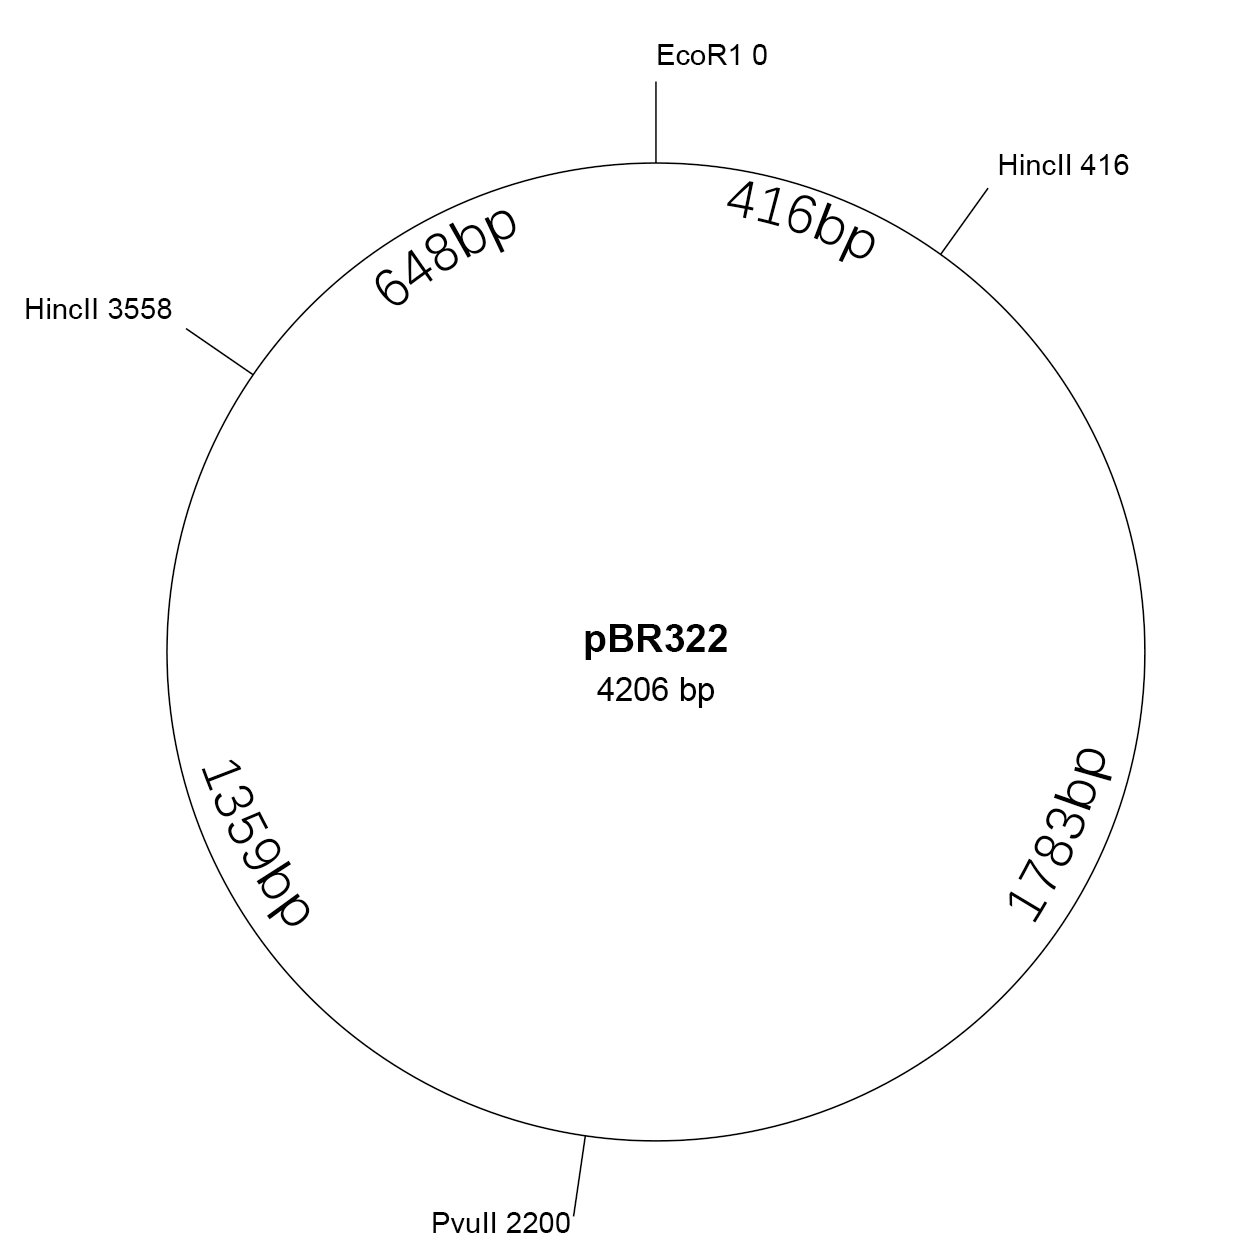
\includegraphics[width = 0.5\linewidth]{../Data/Plasmid/final.png}
                \caption{Mapping Result}
                \label{final.map2}
            \end{figure}
        \subsection{Undigested DNA}
            There are two bands in \textbf{pBR322} tube, and the one with larger travel distance has stronger signal, the one with smaller travel distance has weaker signal. 

            The stronger signal one is the normal circular DNA, with supercoiled conformation, namely, more denser conformation. So it travels fast, regardless of its large number of base pairs. However, the weaker signal one is untwisted, less denser than supercoiled, causing it travel slower.

        \subsection{Conclusion}
            \subsubsection{Common Error}
                \paragraph{Experimental Error} As the electrophoresis does not exactly fit the equation $d \propto \frac{1}{log(n)}$, the distance itself consists of random error, which is inevitable in experiment. If we use wrong amount of reagents, or let reaction running for wrong time, or make mistakes when loading, the experimental error will increase.

                \paragraph{Measurement Error} There is no standard scale in the photo. I measure the distance using software to count the pixels, which will generate random measurement error. However, after measuring for enough times, calculating the average distance can eliminate the random measurement error.

                \paragraph{Linear Fitting Error} The standard curve is a curve, instead of a line. No matter how it looks like a straight line, the true value comes from a curve function. So if we use a linear function to estimate base pairs, there will always be error. Plus, the base pairs are in logarithm scale, which will magnify the small error into large length difference.

            \subsubsection{Further Application}
                At the end of the experiment, we get the locations of 4 restriction sites of 3 enzymes in a plasmid, and also, these fragments with known cohesive ends. We can bind these fragments into other known plasmids to determine what genes are in the fragments. Then, we will get the gene map of the unknown plasmid. This is useful to study a new plasmid or test a newly built plasmid. 

                In genetic engineering, plasmid is an essential tool. If we know more details about the tool, we can do a better job. The mapping, including restriction mapping is the basic process to explore the detail of a plasmid.

\end{document}